\documentclass[a4paper,titlepage]{article}
\usepackage{hyperref}
\usepackage{graphicx}
\usepackage{dingbat}
\usepackage{fancyhdr}
\usepackage{geometry}
\geometry{left=3.0truecm,right=3.0truecm,top=3.0truecm,bottom=3.0truecm} 

\author{David Acreman}
\title{Profiling Firedrake for the APinTA-PDEs project}

\begin{document}
\pagestyle{fancy}
\lhead{}
\chead{}
\rhead{Profiling report}

\maketitle
\pagebreak
\tableofcontents
\pagebreak

%%%%%%%%%%%%%%%%%%%%%%%%%%%%%%%%%%%%%%%%%%%%%%%%%%%%%%%%%%%%%%%%%%%%%%%%%%%%%%%%%%%%%%%%%%%%%%%%%%%%%%%%%%%%%%%%%%%%%%%%%%%%%%%%%%%%%%

\section{Introduction}

In order to understand the performance characteristics of numerical schemes and the impact of potential optimisations it is necessary to gather information beyond simple measures of elapsed run times. A number of profiling tools exist which are capable of gathering performance information from applications parallelised using MPI, for example the time spent in MPI calls and the identification of performance problems such as load imbalance. This document gives an overview of the profiling tools available to the APinTA-PDEs project with a focus on tools which can provide information about MPI communication and related performance issues. 

The Firedrake will be used extensively for development and rapid prototyping work in the course of the project. Firedrake is python-based domain specific language which generates code at run time. These characteristics make integrating Firedrake with profilers more complex than for traditional HPC applications written using C/C++/Fortran which are compiled then run. Although this report primarily focusses on Firedrake the profiling tools evaluated could be used for profiling other codes used by the project even if those tools are not currently suitable for use with Firedrake.

Section~\ref{section:target_platforms} presents the target platforms being considered in this report and reviews the hardware and software available on these systems. Section~\ref{section:test_cases} describes the test cases which will be used to demonstrate the profilers. The profiling tools available to the project are discussed in section \ref{section:profiling_tools} and their capabilities demonstrated with the test cases from section~\ref{section:test_cases}. Section~\ref{section:builds} discusses how to build Firedrake on the target platforms and which profilers the successful builds can be used with. Proof-of-concept results from these profilers are shown in section~\ref{section:profiling_firedrake}. Finally section~\ref{section:conclusions} presents conclusions and recommendations. 

%%%%%%%%%%%%%%%%%%%%%%%%%%%%%%%%%%%%%%%%%%%%%%%%%%%%%%%%%%%%%%%%%%%%%%%%%%%%%%%%%%%%%%%%%%%%%%%%%%%%%%%%%%%%%%%%%%%%%%%%%%%%%%%%%%%%%%

\section{Target platforms}
\label{section:target_platforms}

An overview of the hardware in the target platforms for this project is shown in Table~\ref{tab:hardware}. 
%
\begin{table}[htp]
\begin{center}
\begin{tabular}{|l|l|r|r|l|}
\hline 
System         & Processor        & Cores/node & Memory/node     & Interconnect \\
\hline
Archer-2       & AMD x86\_64         & 128        & 256 GB DRAM  & HPE Cray Slingshot  \\
Isambard XCI   & Thunder X2 ARM64    &  64        & 256 GB DRAM  & Cray Aries          \\
Isca           & Intel x86\_64       & 16/20      & 128 GB DRAM  & Mellanox Infiniband \\
Server         & AMD x86\_64         & 128        & 256 GB DRAM  & None                \\
\hline
\end{tabular}
\end{center}
\caption{Target platform hardware specifications.}
\label{tab:hardware}
\end{table}%
The target HPC platforms are Archer-2 (national tier-1), Isambard (national tier-2) and Isca (local tier-3). Isambard comprises multiple systems and for this project we will focus on the the XCI system which is an established production system based on the ARM64 processor architecture. The project has purchased a local server which is designed to be similar to an Archer compute node, although it will run Ubuntu which will make it easier to build Firedrake. The server can provide a reference installation as it will use an unmodified Firedrake installation, rather than the more customised installations on the HPC platforms which will use non-standard software components, for example MPI libraries and maths libraries.

An overview of the software stacks on the target platforms is shown in Table~\ref{tab:software}. 
\begin{table}[htp]
\begin{center}
\begin{tabular}{|l|l|l|l|l|}
\hline 
System          & Compilers               & MPI libraries  & Maths lib.       & Profilers  \\
\hline
Archer-2        & GNU, Cray, AOCC         & Cray MPICH2     & Cray libsci     & Cray      \\
Isambard XCI    & GNU, Cray, ARM          & Cray MPICH2     & Cray libsci     & Cray, ARM \\
Isca (GCC-foss) & GNU                     & OpenMPI         & OpenBLAS        & None      \\
Isca (Intel)    & Intel                   & Intel           & Intel MKL       & Intel     \\
Server          & GNU                     & MPICH           & OpenBLAS        & None      \\
\hline
\end{tabular}
\end{center}
\caption{Software stacks on target platforms. AOCC is the AMD Optimizing Compiler Collection. Intel MPI and MVAPICH are MPICH derivatives which support an Infiniband interconnect.
The Cray profiler is Cray Performance Analysis Tools (PAT), the ARM profilers are part of the ARM Forge tool suite and the Intel profilers are part of the Intel Parallel Studio suite.}
\label{tab:software}
\end{table}
Each HPC platform has the GNU compilers, compilers from the processor vendor (AMD, Intel, or ARM) and Cray systems also have the Cray compiler. The GNU compilers are the one compiler family which is available on all the target platforms.

On the Cray systems compilation is handled by wrapper scripts from the Cray Programming Environment. The wrapper script can run different compilers depending on which programming environment module is loaded at compile time (e.g. if \texttt{PrgEnv-cray} is loaded then \texttt{cc} calls the Cray C compiler and if \texttt{PrgEnv-gnu} is loaded \texttt{cc} calls the GNU C compiler). The MPI library and maths library (Cray libsci) are then linked by the wrapper script. On Cray systems the standard profiling tool is Cray Performance Analysis Tools (PAT) with the profiling tools from the ARM Forge suite\footnote{ARM Forge was previously known as Allinea Forge} also available on Isambard.

The software environment on Isca is managed using Easybuild\footnote{https://docs.easybuild.io/en/latest/} which has the concept of a toolchain. There are two toolchains on Isca: the GCC-foss toolchain and the Intel toolchain. Each toolchain has a different MPI library and maths library. Intel Parallel Studio has an MPI profiling tool called Intel Trace Analyzer and Collector (ITAC) which works with Intel MPI.

The server does not currently have any profiling software. However the profiling tools from Intel's Parallel Studio product are now available for free as part of the HPC toolkit as part of the newer OneAPI product\footnote{\url{https://software.intel.com/content/www/us/en/develop/tools/oneapi/all-toolkits.html}} and these could be installed on the server. There is also the option of obtaining an evaluation licence for ARM Forge to test these tools on the server. A server licence for the ARM Forge product costs \$USD~425 for a one year academic licence which allows profiling with up to 64 MPI processes\footnote{\url{https://store.developer.arm.com/store/high-performance-computing-hpc-tools/arm-forge}}.

%%%%%%%%%%%%%%%%%%%%%%%%%%%%%%%%%%%%%%%%%%%%%%%%%%%%%%%%%%%%%%%%%%%%%%%%%%%%%%%%%%%%%%%%%%%%%%%%%%%%%%%%%%%%%%%%%%%%%%%%%%%%%%%%%%%%%%

\section{Test cases}
\label{section:test_cases}

The profilers will be tested using three different versions of a Mandelbrot set calculation. The different versions parallelise the calculation in different ways, have different performance characteristics and display different performance issues:
\begin{itemize}
\item Version 1: divides the computational domain into equal sized chunks along the real axis. Dividing the workload in this manner causes a load imbalance as some sub-domains will complete significantly more iterations than others (see figure~\ref{fig:mandelbrot_dd})
\item Version 2: similar to version 1 but interleaves the iterations on the real axis to improve the load balance. Both version 2 and version 1 pack a 2D array into a 1D buffer which is communicated using an \verb+MPI_Reduce+. Even when the program is run on a single compute node (where MPI communication is quick) there will be an overhead from packing and unpacking the buffer.
\item Version 3: implements a manager-worker pattern for distributing the iterations to ensure good load balancing. This version also replaces the \verb+MPI_Reduce+ with point-to-point communication between the manager process and the worker processes. The manager process does not perform any calculations which adversely affects performance with small numbers of MPI processes. However this version avoids calling \verb+MPI_Reduce+ and scales better to larger numbers of MPI processes than the other versions .
\end{itemize}
\begin{figure}[htbp]
\begin{center}
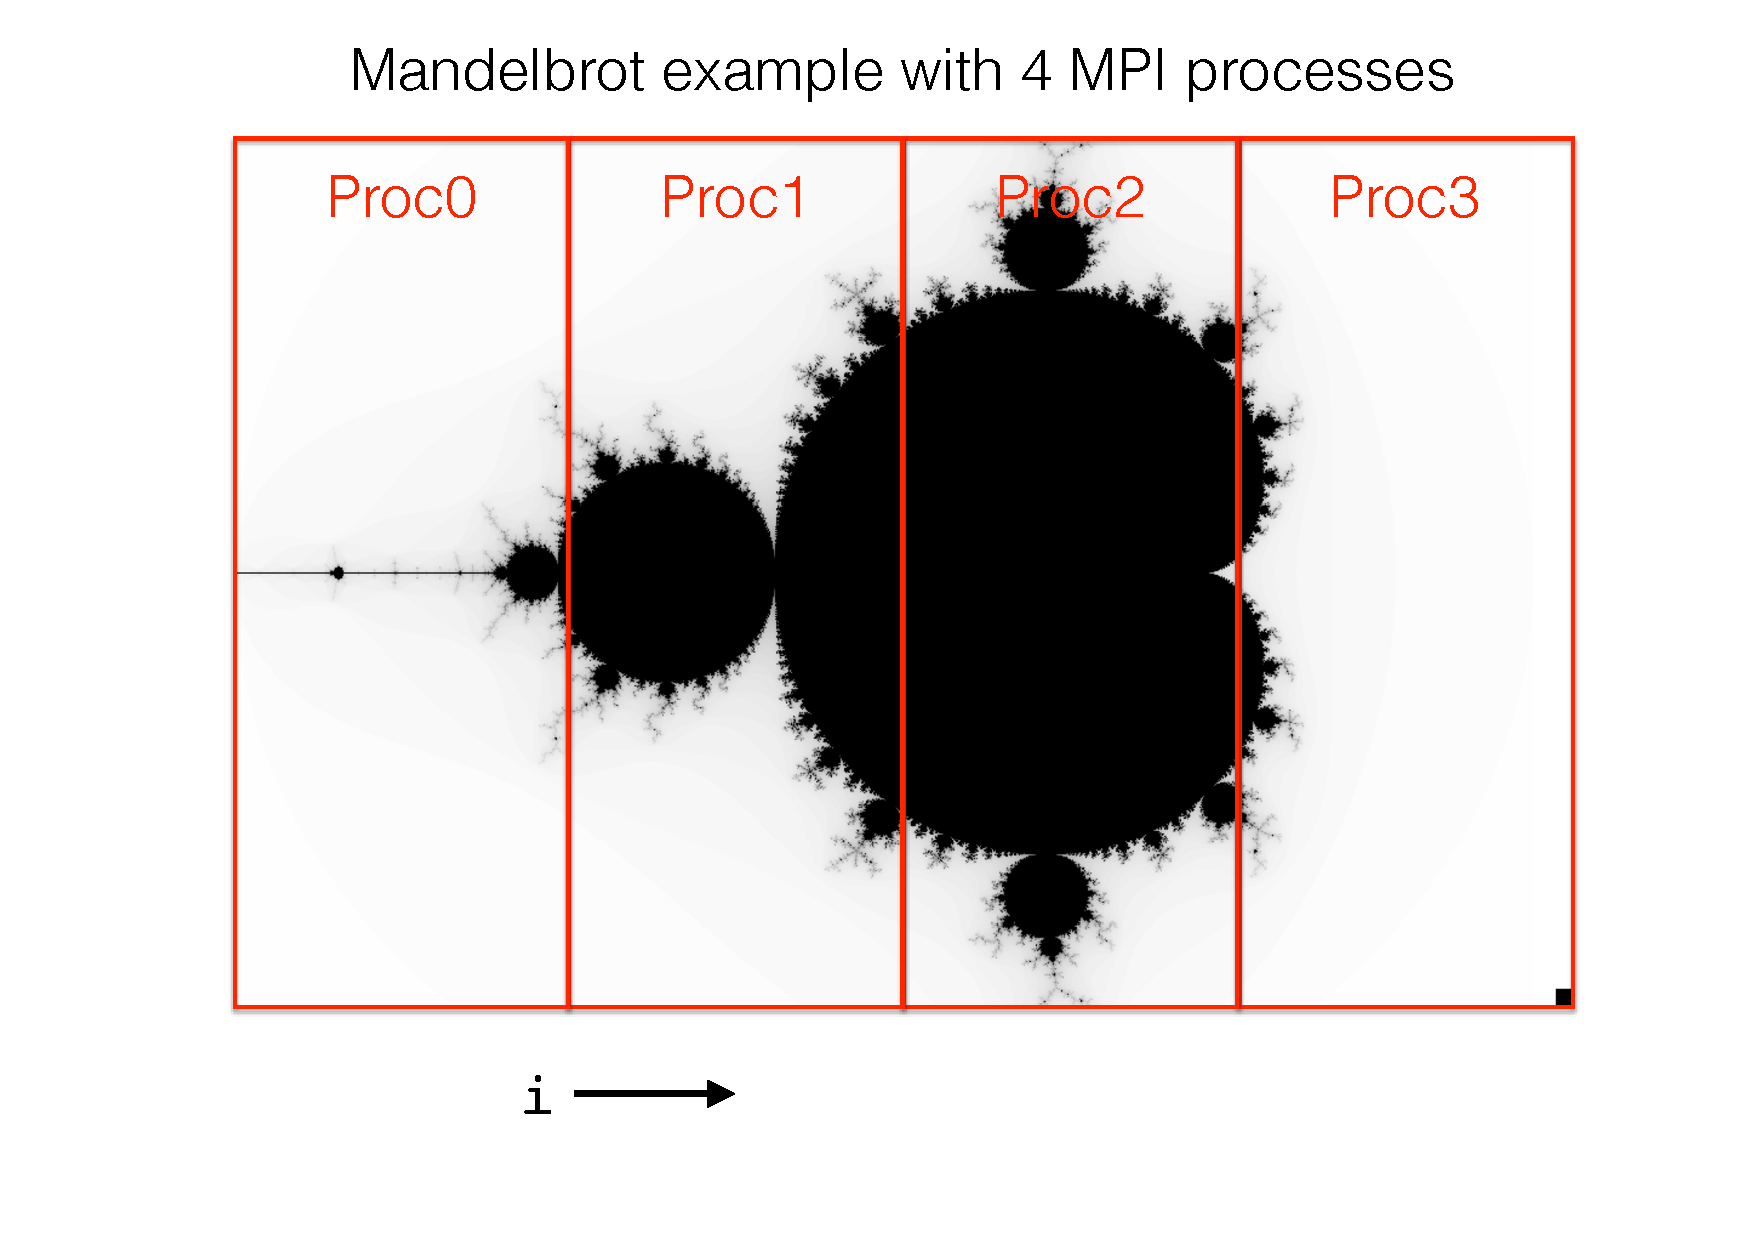
\includegraphics[scale=0.5]{figures/mandelbrot_dd}
\caption{Domain decomposition in version 1 of the Mandelbrot program with four MPI processes. Darker colours show regions of the domain where more iterations are required illustrating the load-imbalance from this decomposition (e.g. process 2 will carry out many more iterations than process 0 or 3).}
\label{fig:mandelbrot_dd}
\end{center}
\end{figure}

The following tests will be used to demonstrate the profiling tools:
\begin{itemize}
\item Test 1: version 1, no I/O, 4 MPI processes
\item Test 2: version 1, with I/O, 4 MPI processes
\item Test 3: version 2, no I/O, 4 MPI processes
\item Test 4: version 3, no I/O, 4 MPI processes
\item Test 5: version 3, no I/O, 16 MPI processes 
\end{itemize}
Comparing test 1 and test 2 shows the impact of I/O. The I/O comprises process 0 writing values to an ASCII file which adds a significant overhead which will show up in the profiling output. Comparing tests 1 and test 3 and shows the impact of load imbalance, as the only difference between these tests is the distribution of the workload. 
Tests 4 and 5 have been designed to illustrate a different communication pattern (manager-worker) and a different type of MPI call (point-to-point rather than collectives). 
The manager-worker pattern is relatively inefficient with 4 MPI processes (test 4) as one process is the manager which does not participate in the calculation but shows much better efficiency with 16 MPI processes (test 5). 

%%%%%%%%%%%%%%%%%%%%%%%%%%%%%%%%%%%%%%%%%%%%%%%%%%%%%%%%%%%%%%%%%%%%%%%%%%%%%%%%%%%%%%%%%%%%%%%%%%%%%%%%%%%%%%%%%%%%%%%%%%%%%%%%%%%%%%

\section{Profiling tools}
\label{section:profiling_tools}

Some performance information can be obtained by using functionality already available in Firedrake. Performance information can be obtained from PETSc (by adding the \verb+-log_view+ flag when running Firedrake\footnote{\url{https://petsc.org/release/documentation/manual/profiling/}}) and there is also the ability to time sections of code by adding a PyOP2 timed stage\footnote{\url{https://op2.github.io/PyOP2/profiling.html}}. These options will be available on all platforms when Firedrake is the target application but the rest of this report will look at how the external profilers already installed on the target platforms can be used to obtain extra information. 

There are three different profilers installed on the target platforms with different platforms having different profiling tools available:
%
\begin{itemize}
\item Intel Parallel Studio: Isca only (requires Intel MPI)
\item ARM Forge: Isambard only (currently only licensed on Isambard)
\item Cray PAT: Isambard and Archer (Cray systems only)
\end{itemize}
%
Each of these products is a suite of tools with a range of capabilities. This report will focus on the tools appropriate for understanding the performance of parallel applications which use MPI.

%---------------------------------------------------------------------------------------------------------------------

\subsection{Intel Parallel Studio}

The MPI profiler in Intel Parallel Studio is called Intel Trace Analyzer and Collector (ITAC). Other profiling tools are available, which provide information on node-level performance for example, but the focus of this report is on MPI performance so ITAC is the tool under consideration.

In the following examples the Mandelbrot executable will be build with MPI tracing enabled as follows. Firstly load the modules for the Intel compilers and ITAC: 
\begin{verbatim}
> module load intel/2017b
> module load itac/2017.1.024
\end{verbatim}
Then compile the executable with \texttt{-trace} flag:
\begin{verbatim}
> mpicc -trace -o mandelbrot mandelbrot_mpi.c
\end{verbatim}
(including the \verb+-g+ flag enables function level information to be obtained but it not required). The \texttt{itac} module needs to be loaded in the job script (in addition to the \texttt{intel} module) but no other modifications are required to the job script. When the job runs a number of additional files are generated, including a file with a \texttt{.stf} extension which is the trace file.
The profiling output can be viewed opening the trace file with the Trace Analyzer graphical interface:
\begin{verbatim}
> traceanalyzer.bin mandelbrot_mpi.stf &
\end{verbatim}

\noindent
\textbf{Test 1:} 
Figure~\ref{fig:test1_ITAC_summary} (top) shows the opening summary page for test 1 (Mandelbrot version 1, no I/O, 4 MPI processes).
\begin{figure}[htbp]
\begin{center}
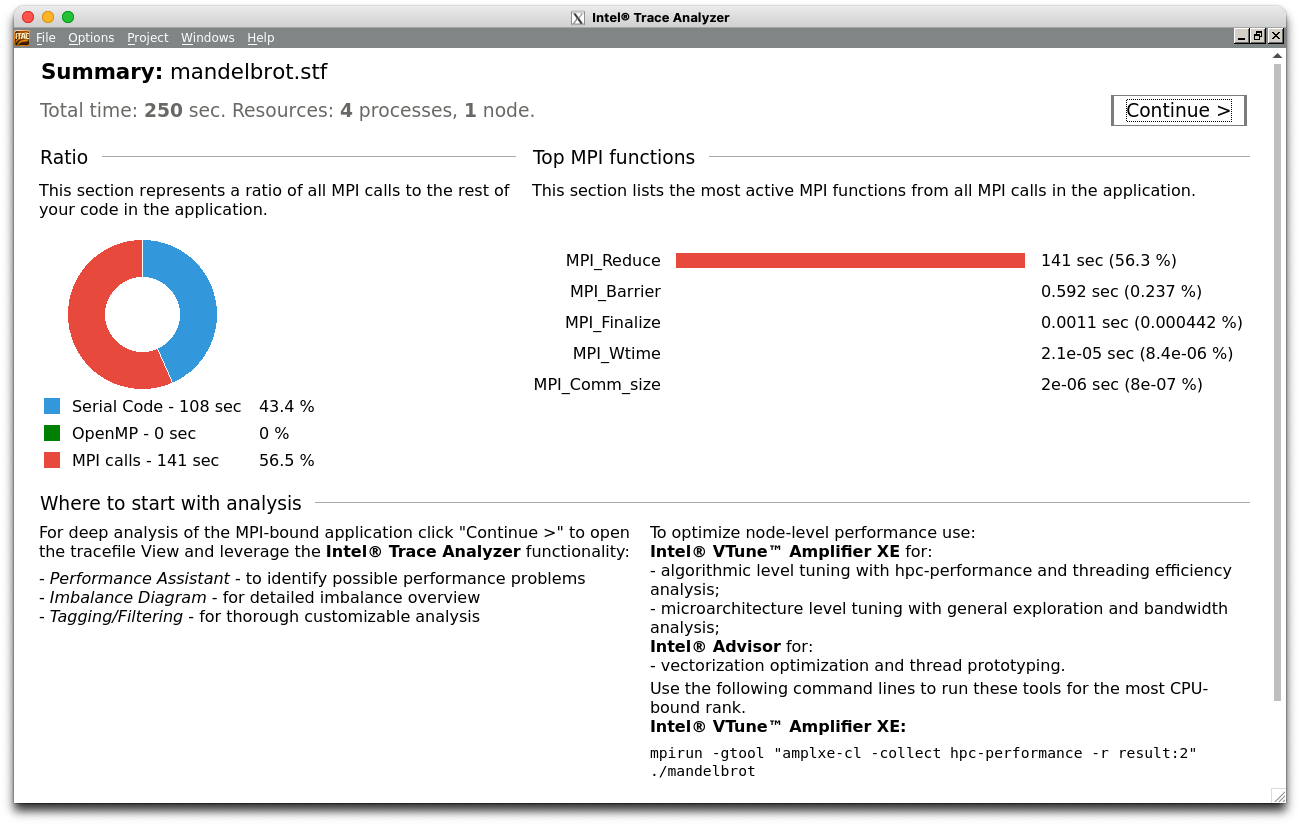
\includegraphics[scale=0.3]{figures/test1_summary}
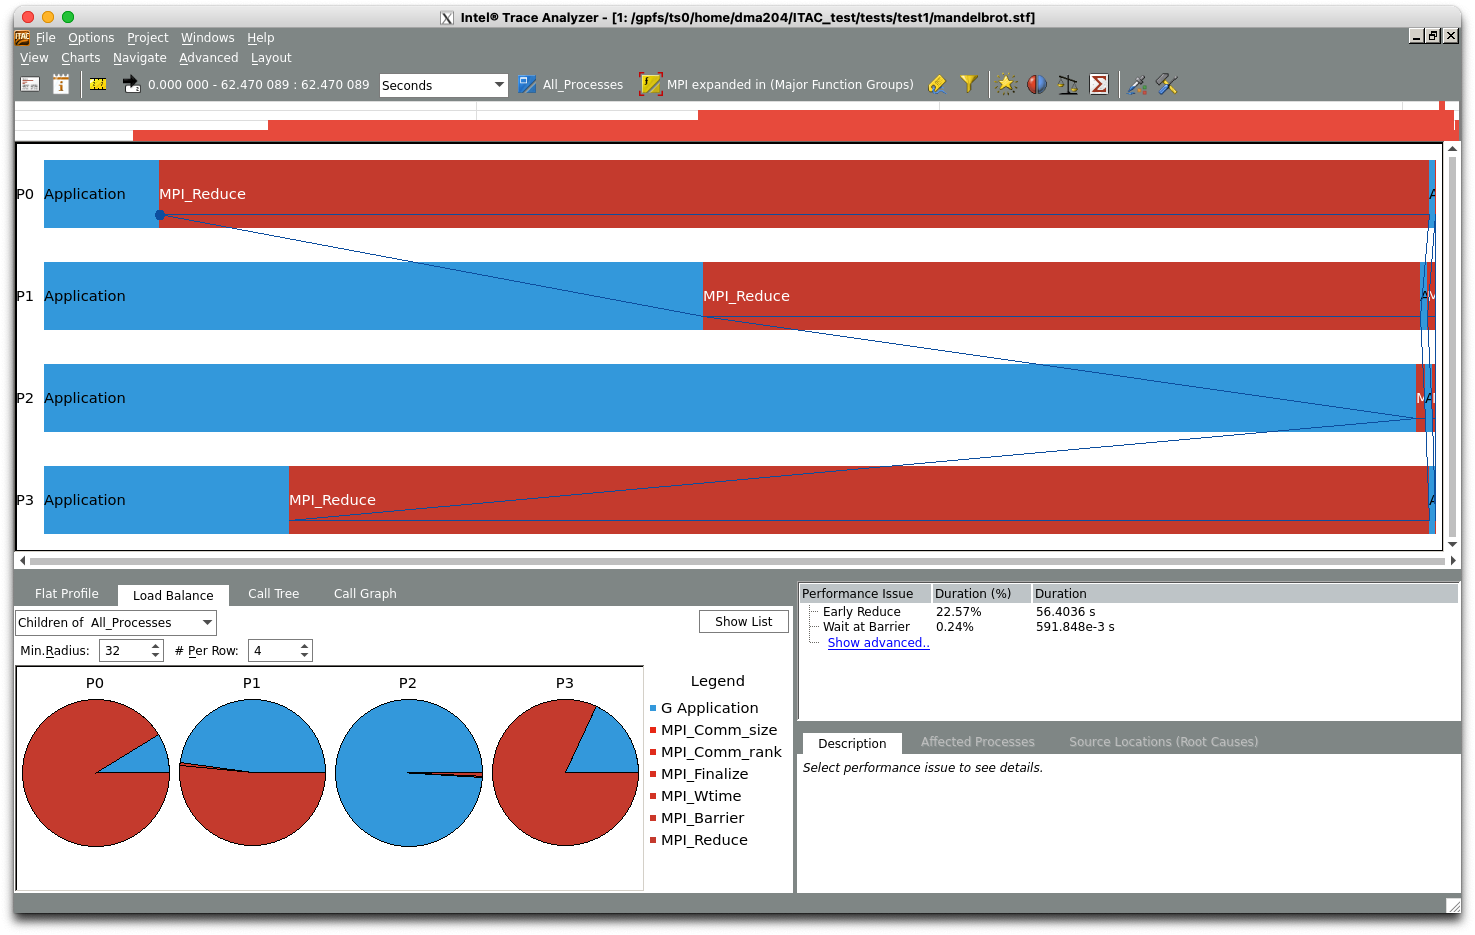
\includegraphics[scale=0.3]{figures/test1_eventTimeline}
\caption{Intel Trace Analyzer plots for test 1. On the summary page (top) the load imbalance shows up as a large fraction of time spent in \texttt{MPI\_Reduce}. The event timeline (bottom) shows that process 2 takes longer than the other processes to complete its iterations which results in the other processes waiting at the \texttt{MPI\_Reduce} call.}
\label{fig:test1_ITAC_summary}
\end{center}
\end{figure}
This test has a load imbalance which is seen as a large fraction (56\%) of time spent in \texttt{MPI\_Reduce}. The reduce itself is not time consuming (all communication takes place on the same compute node) but this is the blocking collective where the MPI processes synchronise. This can be seen in the lower panel of figure~\ref{fig:test1_ITAC_summary} which shows the event timeline. To view the event timeline as seen in this figure:
\begin{itemize}
\item Click the continue button on the summary page
\item Select \texttt{Charts} $\rightarrow$ \texttt{Event Timeline} to open a new pane showing process activity over time.
\item In the lower left pane select the \texttt{Load Balance} tab and click the \texttt{Show pies} button. 
\item Right click on a red MPI section in the timeline and choose \texttt{Ungroup MPI} from the drop down menu
\end{itemize}
The timeline shows that process 2 is taking much longer to complete its iterations than the other processes which has resulted in processes 0, 1 and 3 waiting at the \verb+MPI_Reduce+ call. \\

\noindent
\textbf{Test 2:} this test is similar to test 1 but has I/O enabled. The summary page (see figure~\ref{fig:test2_ITAC_summary}) shows a significantly longer runtime (450s vs. 250s) and significant time spent in \verb+MPI_Barrier+. 
\begin{figure}[htbp]
\begin{center}
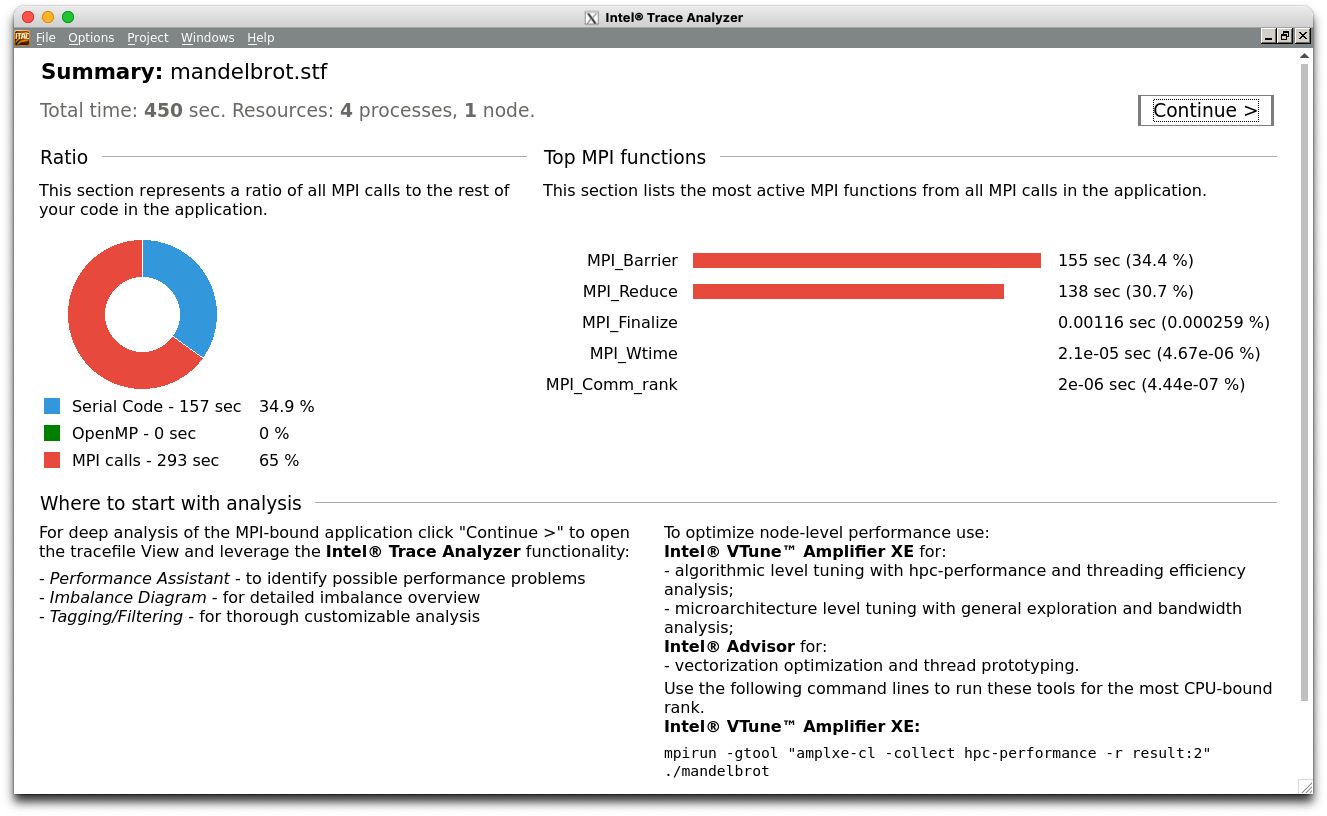
\includegraphics[scale=0.3]{figures/test2_summary}
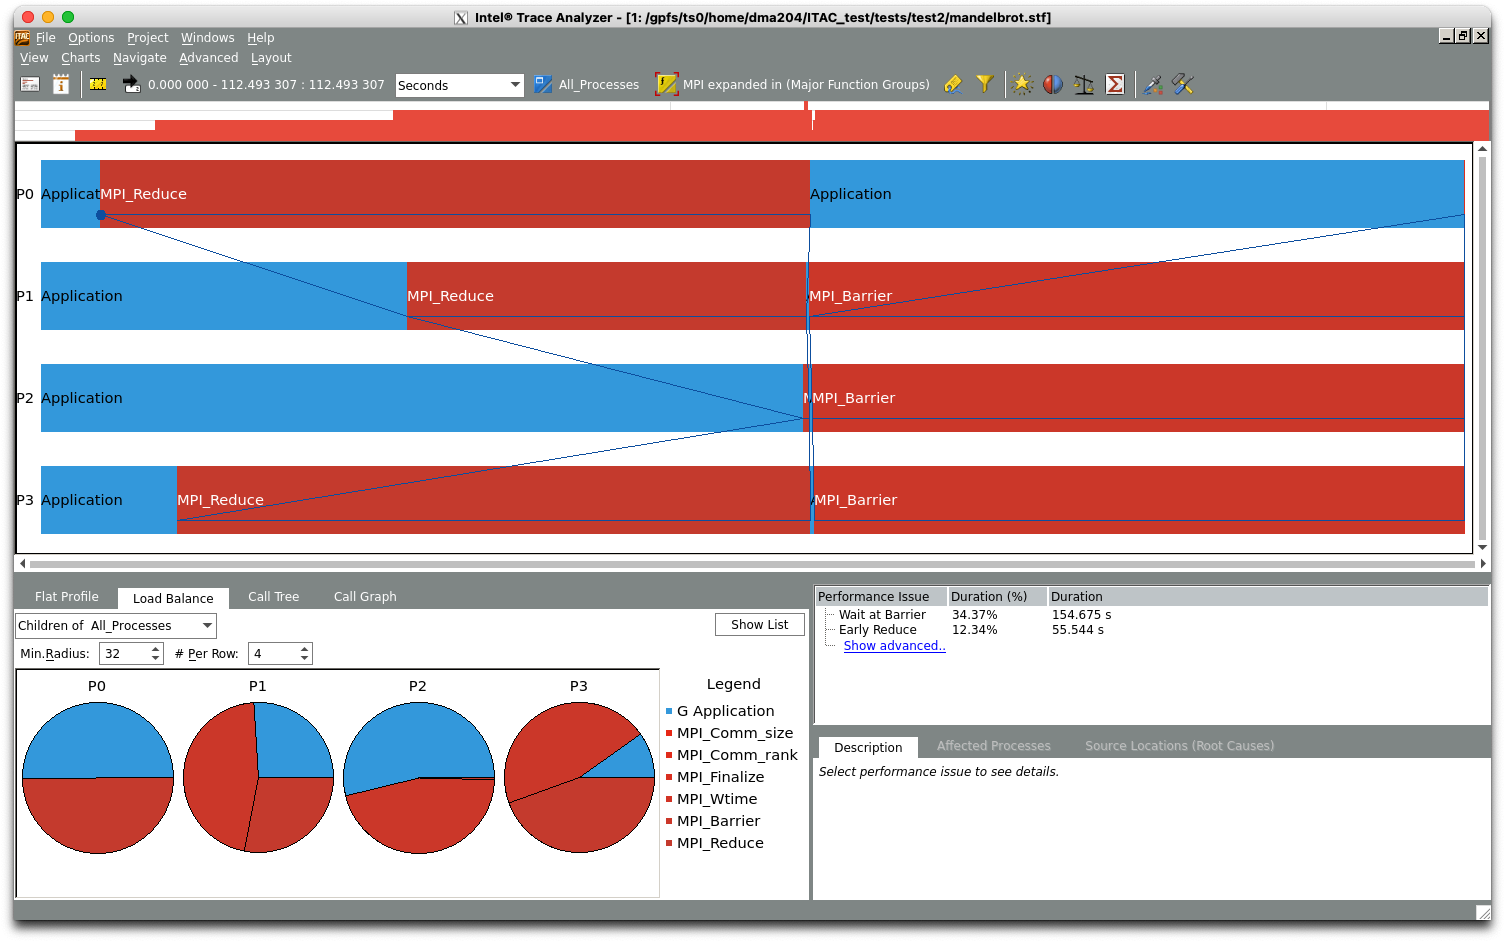
\includegraphics[scale=0.3]{figures/test2_eventTimeline}
\caption{Intel Trace Analyzer plots for test 2 which is like test 1 but with I/O enabled. There are two distinct phases to the time line: firstly the calculation and secondly the I/O. Both phases have a load imbalance with the second phase showing processes waiting at a barrier as the rank zero process performs I/O.}
\label{fig:test2_ITAC_summary}
\end{center}
\end{figure}
The I/O is carried by process 0 which causes all the other processes to wait at an \verb+MPI_barrier+ at the end of the program (processes are synchronised at a barrier before a final run time is reported by process 0). The effect of switching on I/O has been to introduce another load imbalance, this time with process 0 working and all other processes waiting. This can be seen clearly in the timeline where there are two distinct phases both of which have a load imbalance. \\

\noindent
\textbf{Test 3:} this test uses version 2 of the program which has corrected the load imbalance and the profiling results are shown in figure~\ref{fig:test3_ITAC_summary}.
\begin{figure}[htbp]
\begin{center}
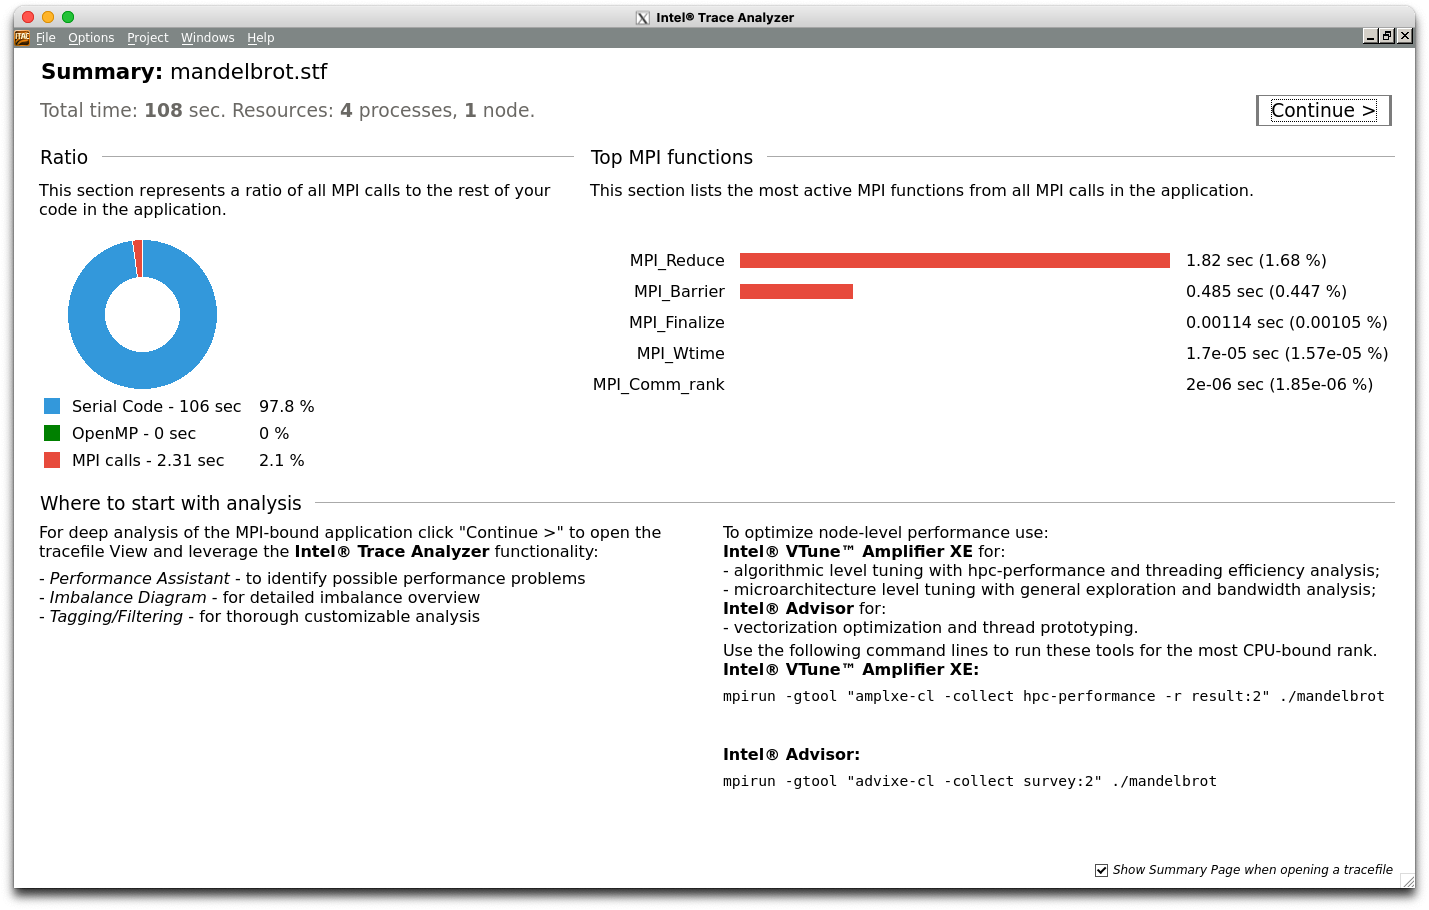
\includegraphics[scale=0.3]{figures/test3_summary}
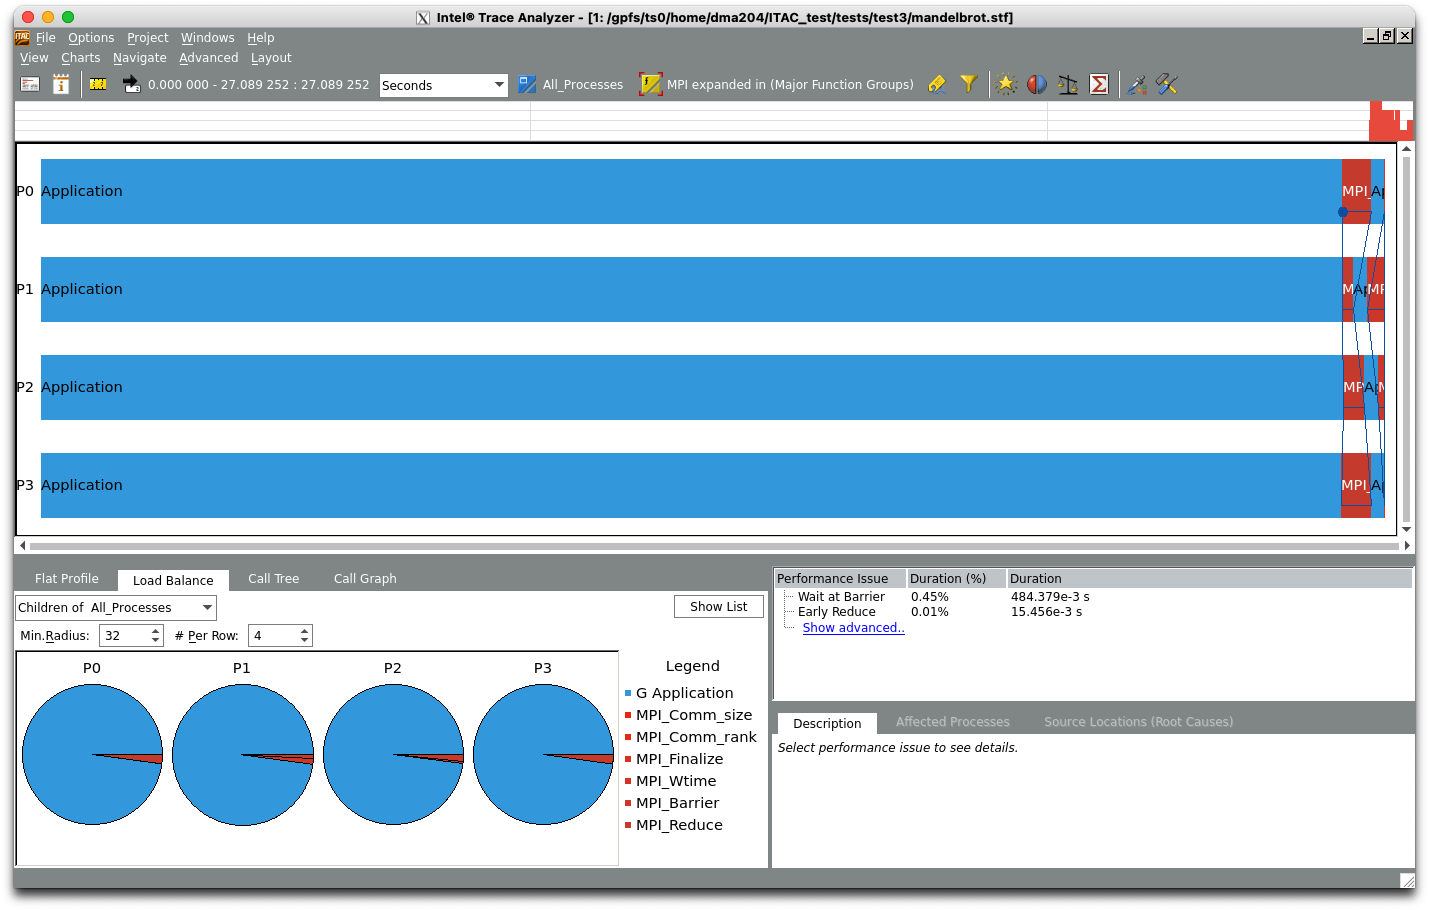
\includegraphics[scale=0.3]{figures/test3_eventTimeline}
\caption{Intel Trace Analyzer plots for test 3. This test uses version 2 of the program which has corrected the load imbalance present in version 1 resulting in all MPI processes reaching the \texttt{MPI\_Reduce} together.}
\label{fig:test3_ITAC_summary}
\end{center}
\end{figure}
The run time is now significantly reduced (108 seconds vs. 250 seconds) and the time line shows the MPI processes reaching the \verb+MPI_Reduce+ together. At the end of the time line we can see some time spent carrying out the \verb+MPI_Reduce+ and some application time (blue) as the buffer is unpacked (if required the time line can be zoomed-in to show more detail in a selected region). \\

\noindent
\textbf{Test 4:} this test uses version 3 of the Mandelbrot program which parallelises the workload using a manager-worker pattern to ensures good load balancing by distributing work at run-time.
\begin{figure}[htbp]
\begin{center}
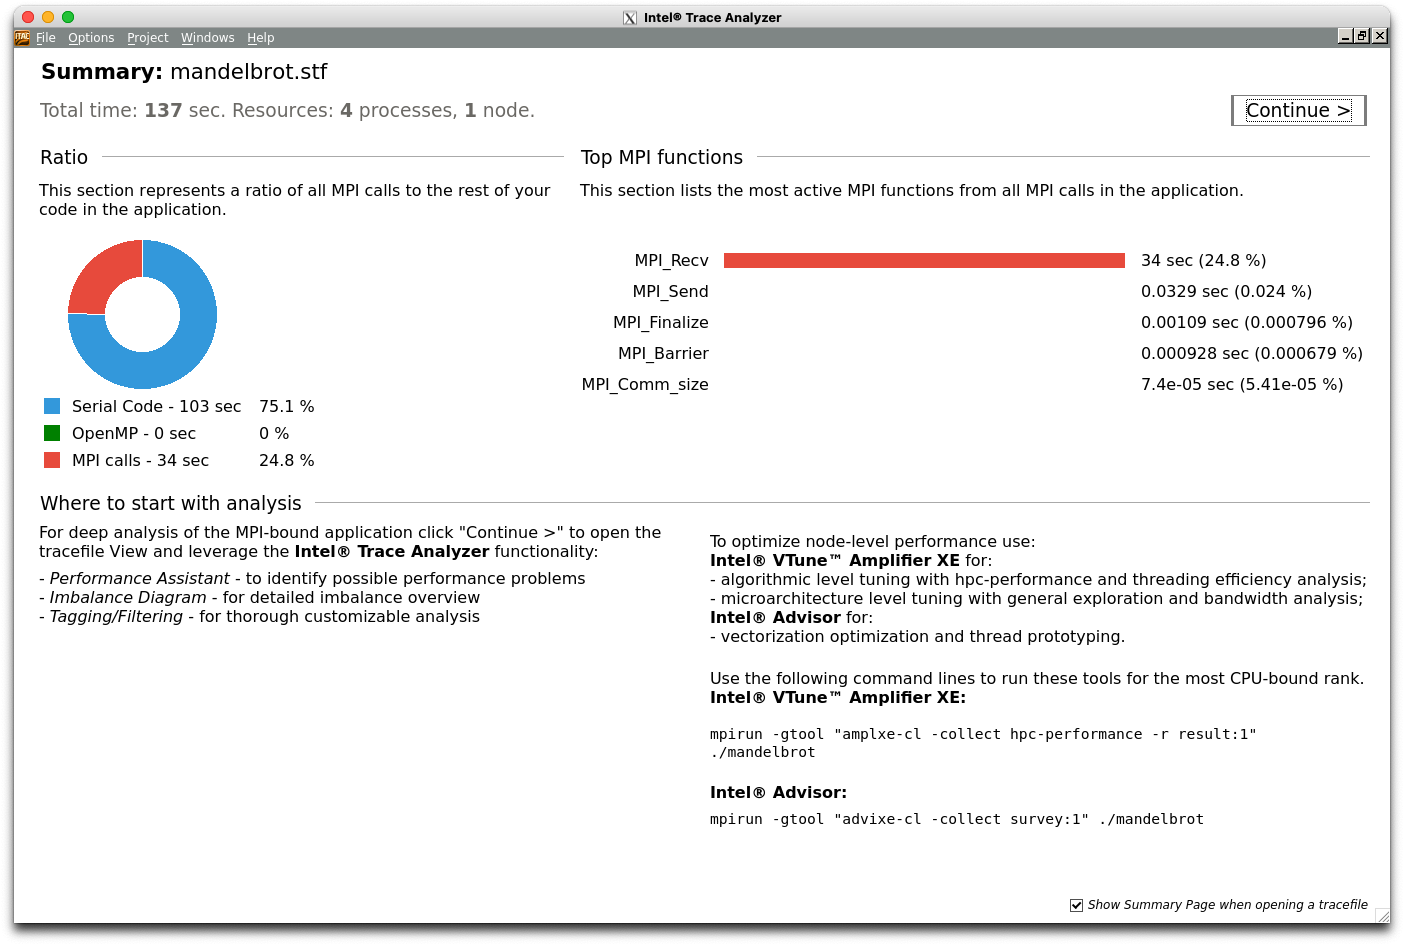
\includegraphics[scale=0.3]{figures/test4_summary}
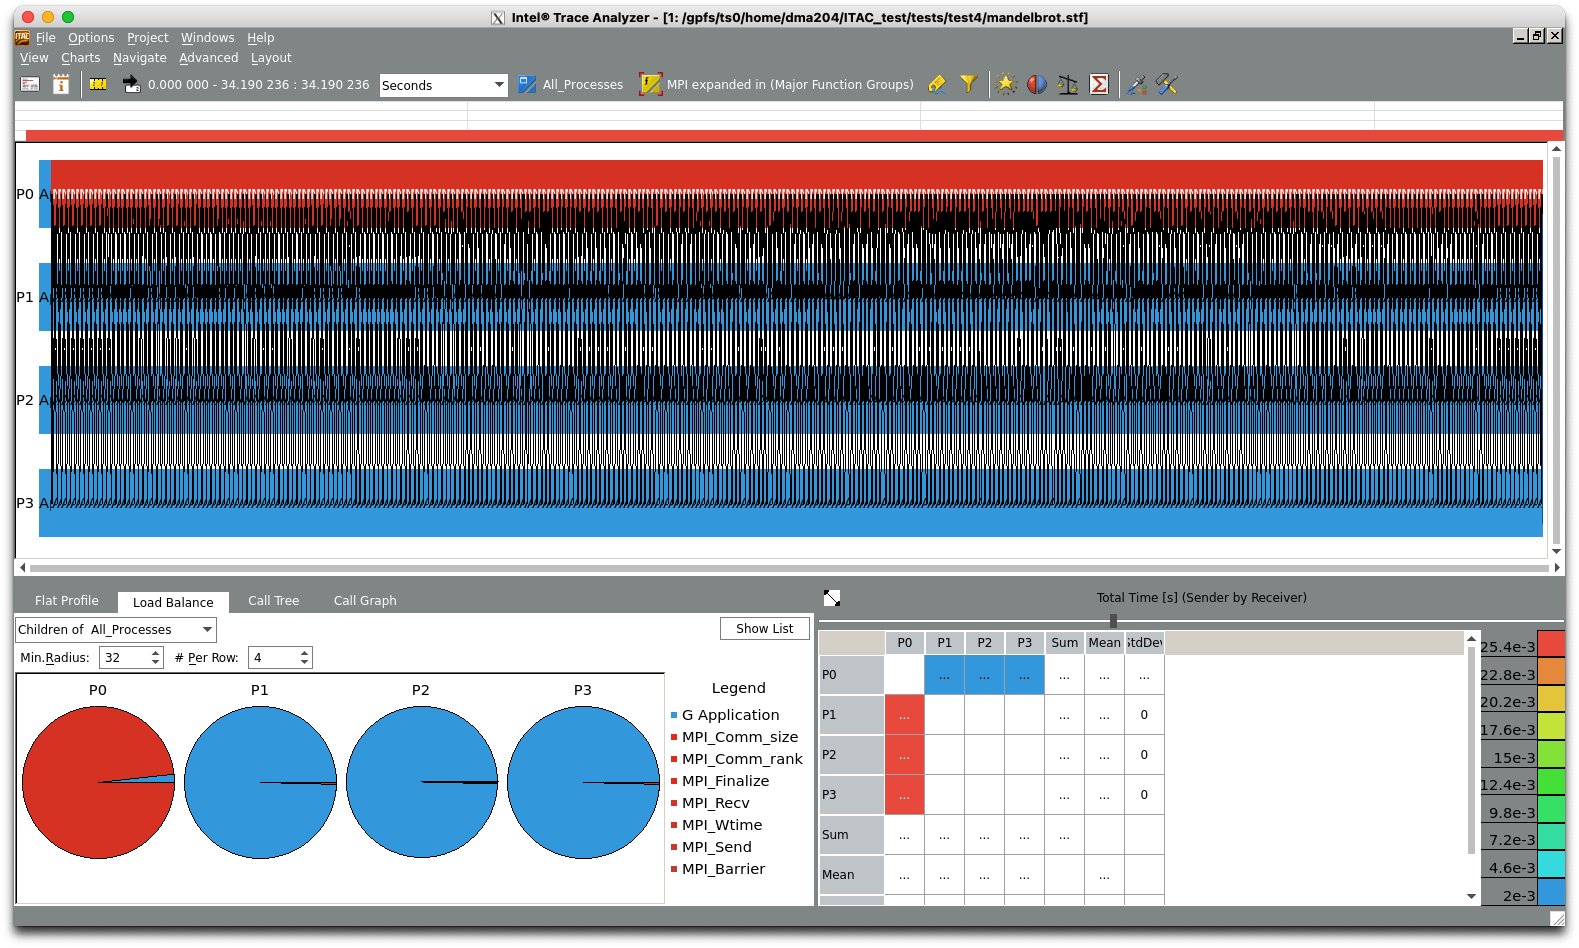
\includegraphics[scale=0.3]{figures/test4_eventTimeline}
\caption{Intel Trace Analyzer plots for test 4. This test uses version 3 of the Mandelbrot program which parallelises the workload using a manager-worker pattern. In this example the communication takes place with a larger number of point-to-point operations instead of a single collective operation.}
\label{fig:test4_ITAC_summary}
\end{center}
\end{figure}
The summary page shows a large fraction of time spent in v\verb+MPI_Recv+ (24.8\%) due to the manager process waiting to hand out work to worker processes. In this test there are only 4~MPI processes so this constitutes a large fraction of the total run time. The time line shows the worker processes (processes 1--3) completing together with negligible time spent in the final \verb+MPI_Barrier+. The communication in this version of the program takes place with a large number of point-to-point operations instead of a single collective operation and the time line shows black lines connecting processes when they communicate. The lower right panel of the bottom figure is a message profile which shows which processes communicate using point-to-point operations (To view the message profile select: \texttt{Charts} $\rightarrow$ \texttt{message profile}). In the manager-worker pattern all the workers communicate only with the manger process so the communcation is seen in the first row and first column of the message profile diagram. \\

\noindent
\textbf{Test 5:} this test uses version 3 of the Mandelbrot program (manager-worker) as for the previous test but uses 16~MPI processes instead of 4~MPI processes. The time spent in \verb+MPI_Reduce+ is now much smaller (6.24\%) consistent with slightly less than $1/16$ of the run time (i.e. one manager process out of a total of 16~processes). 
\begin{figure}[htbp]
\begin{center}
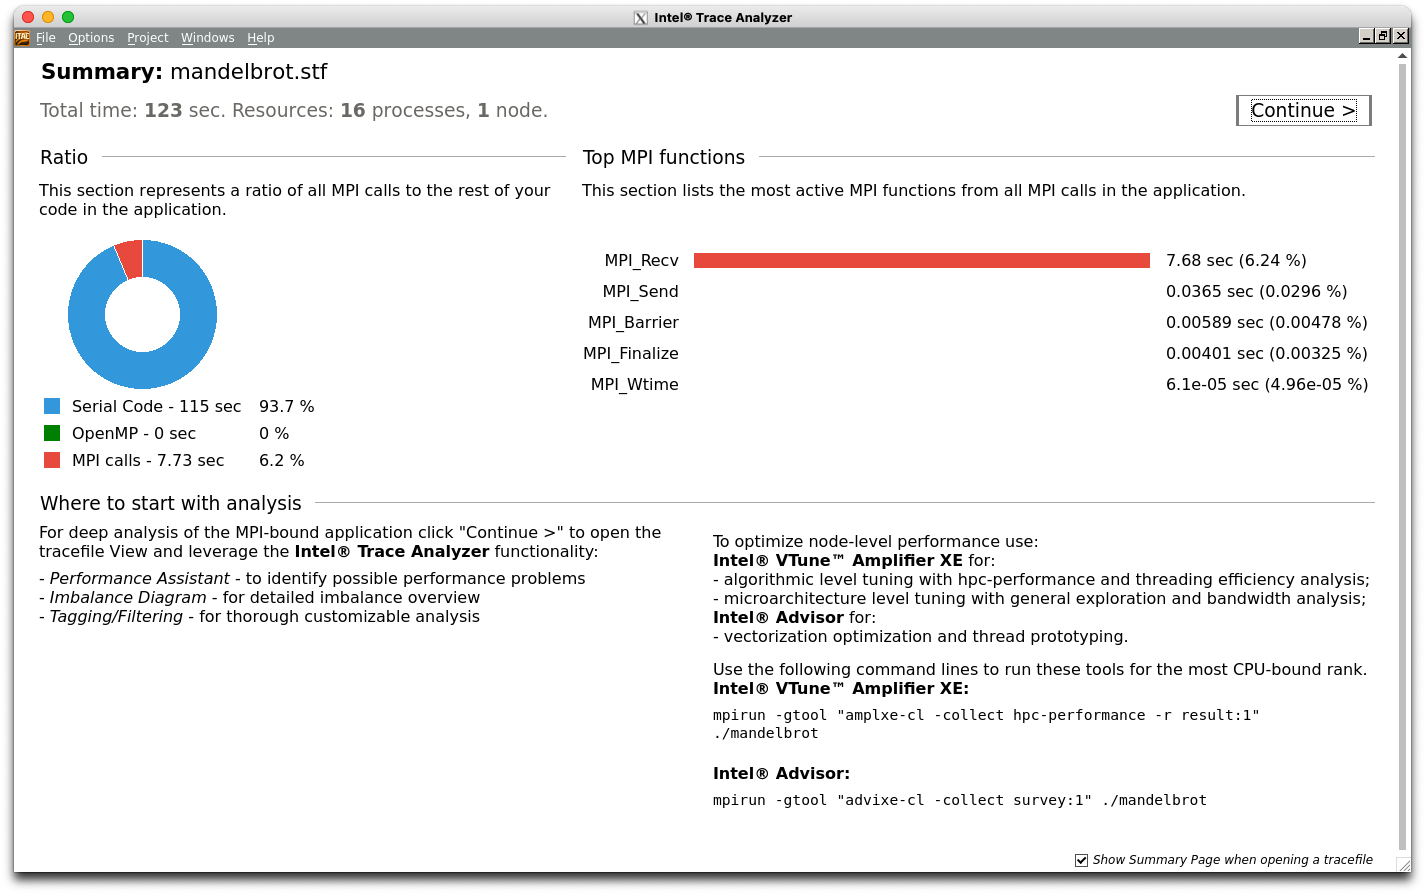
\includegraphics[scale=0.3]{figures/test5_summary}
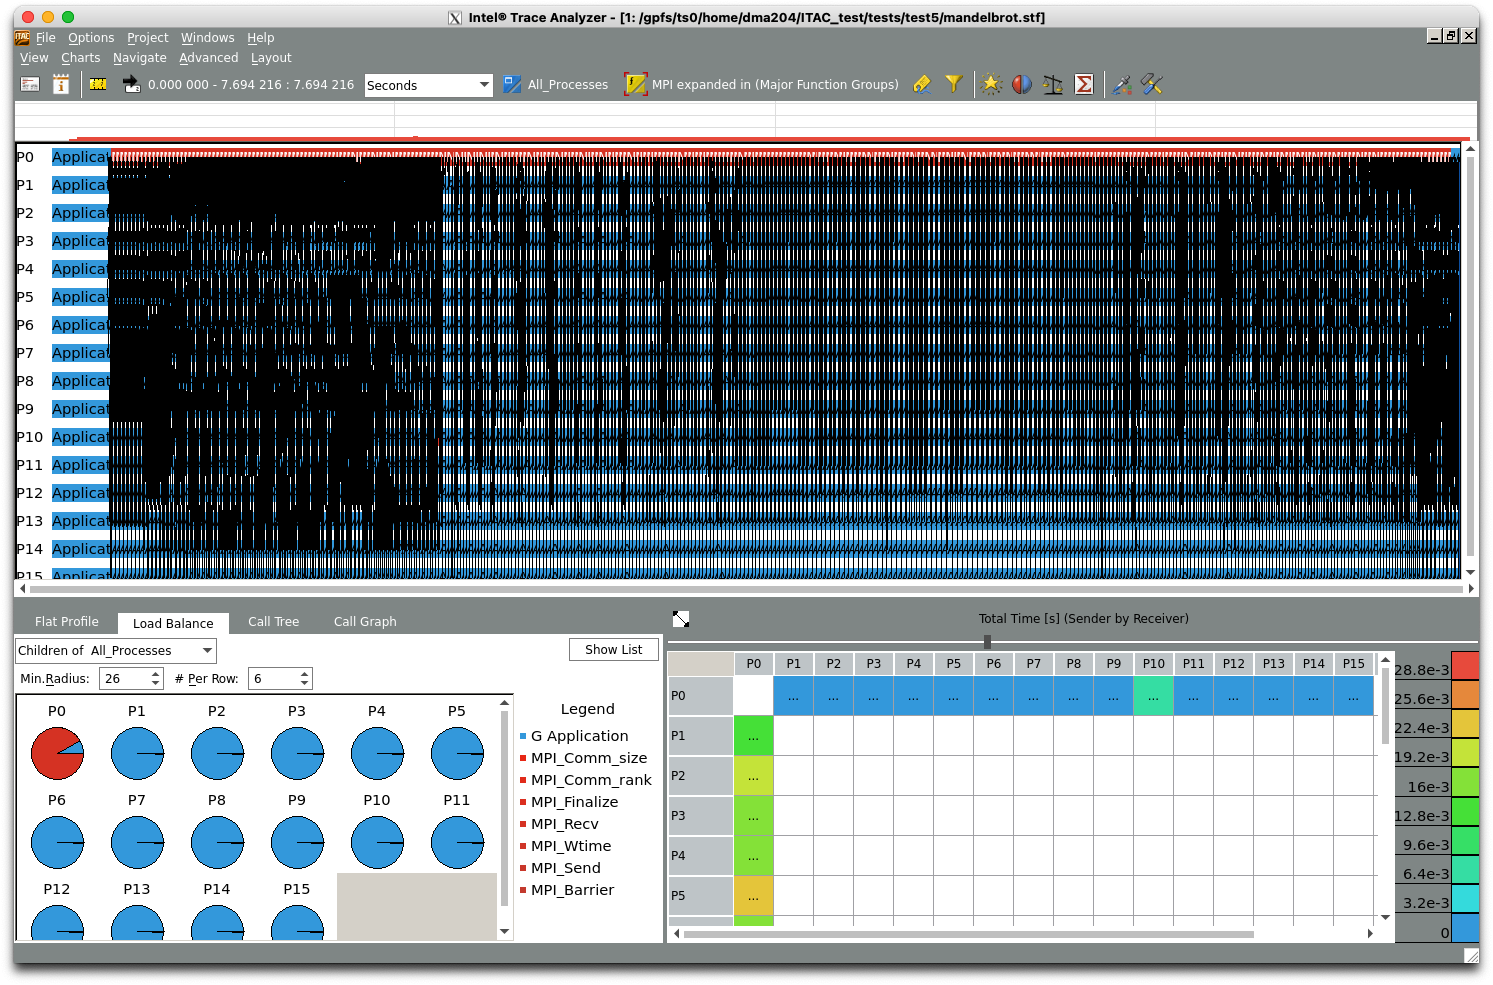
\includegraphics[scale=0.3]{figures/test5_eventTimeline}
\caption{Intel Trace Analyzer plots for test 5. This test uses version 3 of the Mandelbrot program (manager-worker) as for the previous test but uses 16~MPI processes instead of 4~MPI processes.}
\label{fig:test5_ITAC_summary}
\end{center}
\end{figure}
The point-to-point communication between processes is seen to be most intense at the start of the calculation, when each unit of work is completed quickly, with less communication in the middle of the time line when each point takes longer to calculate. 

\pagebreak
%---------------------------------------------------------------------------------------------------------------------

\subsection{ARM Forge}

The ARM Forge suite of development tools is available on the Isambard system. ARM Forge includes two performance tools: ``Performance Reports'' and ``MAP''. Performance Reports gives a one page summary of an application's performance. MAP is a profiler for more in-depth analysis which can profile C++, C, Fortran and Python\footnote{\url{https://www.arm.com/products/development-tools/server-and-hpc/forge/map}}. 

\subsubsection{Performance Reports}

The documentation for Performance Reports says that on Cray systems dynamic linking or explicit linking with the profiling libraries is required\footnote{\url{https://developer.arm.com/documentation/101136/2102/Performance-Reports/Get-started-with-Performance-Reports/Compile-on-Cray-X-series-systems}}. However in the latest Cray compilers dynamic linking is the default so no changes are required to the build process. The following shows an example session and output from Performance Reports on the Isambard XCI system.

No changes are required at compile time so to compile an executable using the GCC compiler for example:
\begin{verbatim}
> module switch PrgEnv-cray PrgEnv-gnu
> cc -o mandelbrot mandelbrot_mpi.c
\end{verbatim}
Two changes are required in the job script in order to activate performance reports. The first change is to load the \texttt{arm-forge} module:
\begin{verbatim}
module load tools/arm-forge
\end{verbatim}
and the second change is to add the \texttt{perf-report} command before the \texttt{aprun} command e.g. replace
\begin{verbatim}
aprun -n ${nprocs} ./mandelbrot
\end{verbatim}
with
\begin{verbatim}
perf-report aprun -n ${nprocs} ./mandelbrot
\end{verbatim}
This method of launching a job under perf-report is referred to as Express Launch mode in the documentation.
%
When the job runs two extra files are generated which contain the output from the performance report in text and HTML formats. \\

\noindent
\textbf{Test 1:} the output from running a performance report on test 1 is shown in figure~\ref{fig:perf-report_MB1}.
%
\begin{figure}[htbp]
\begin{center}
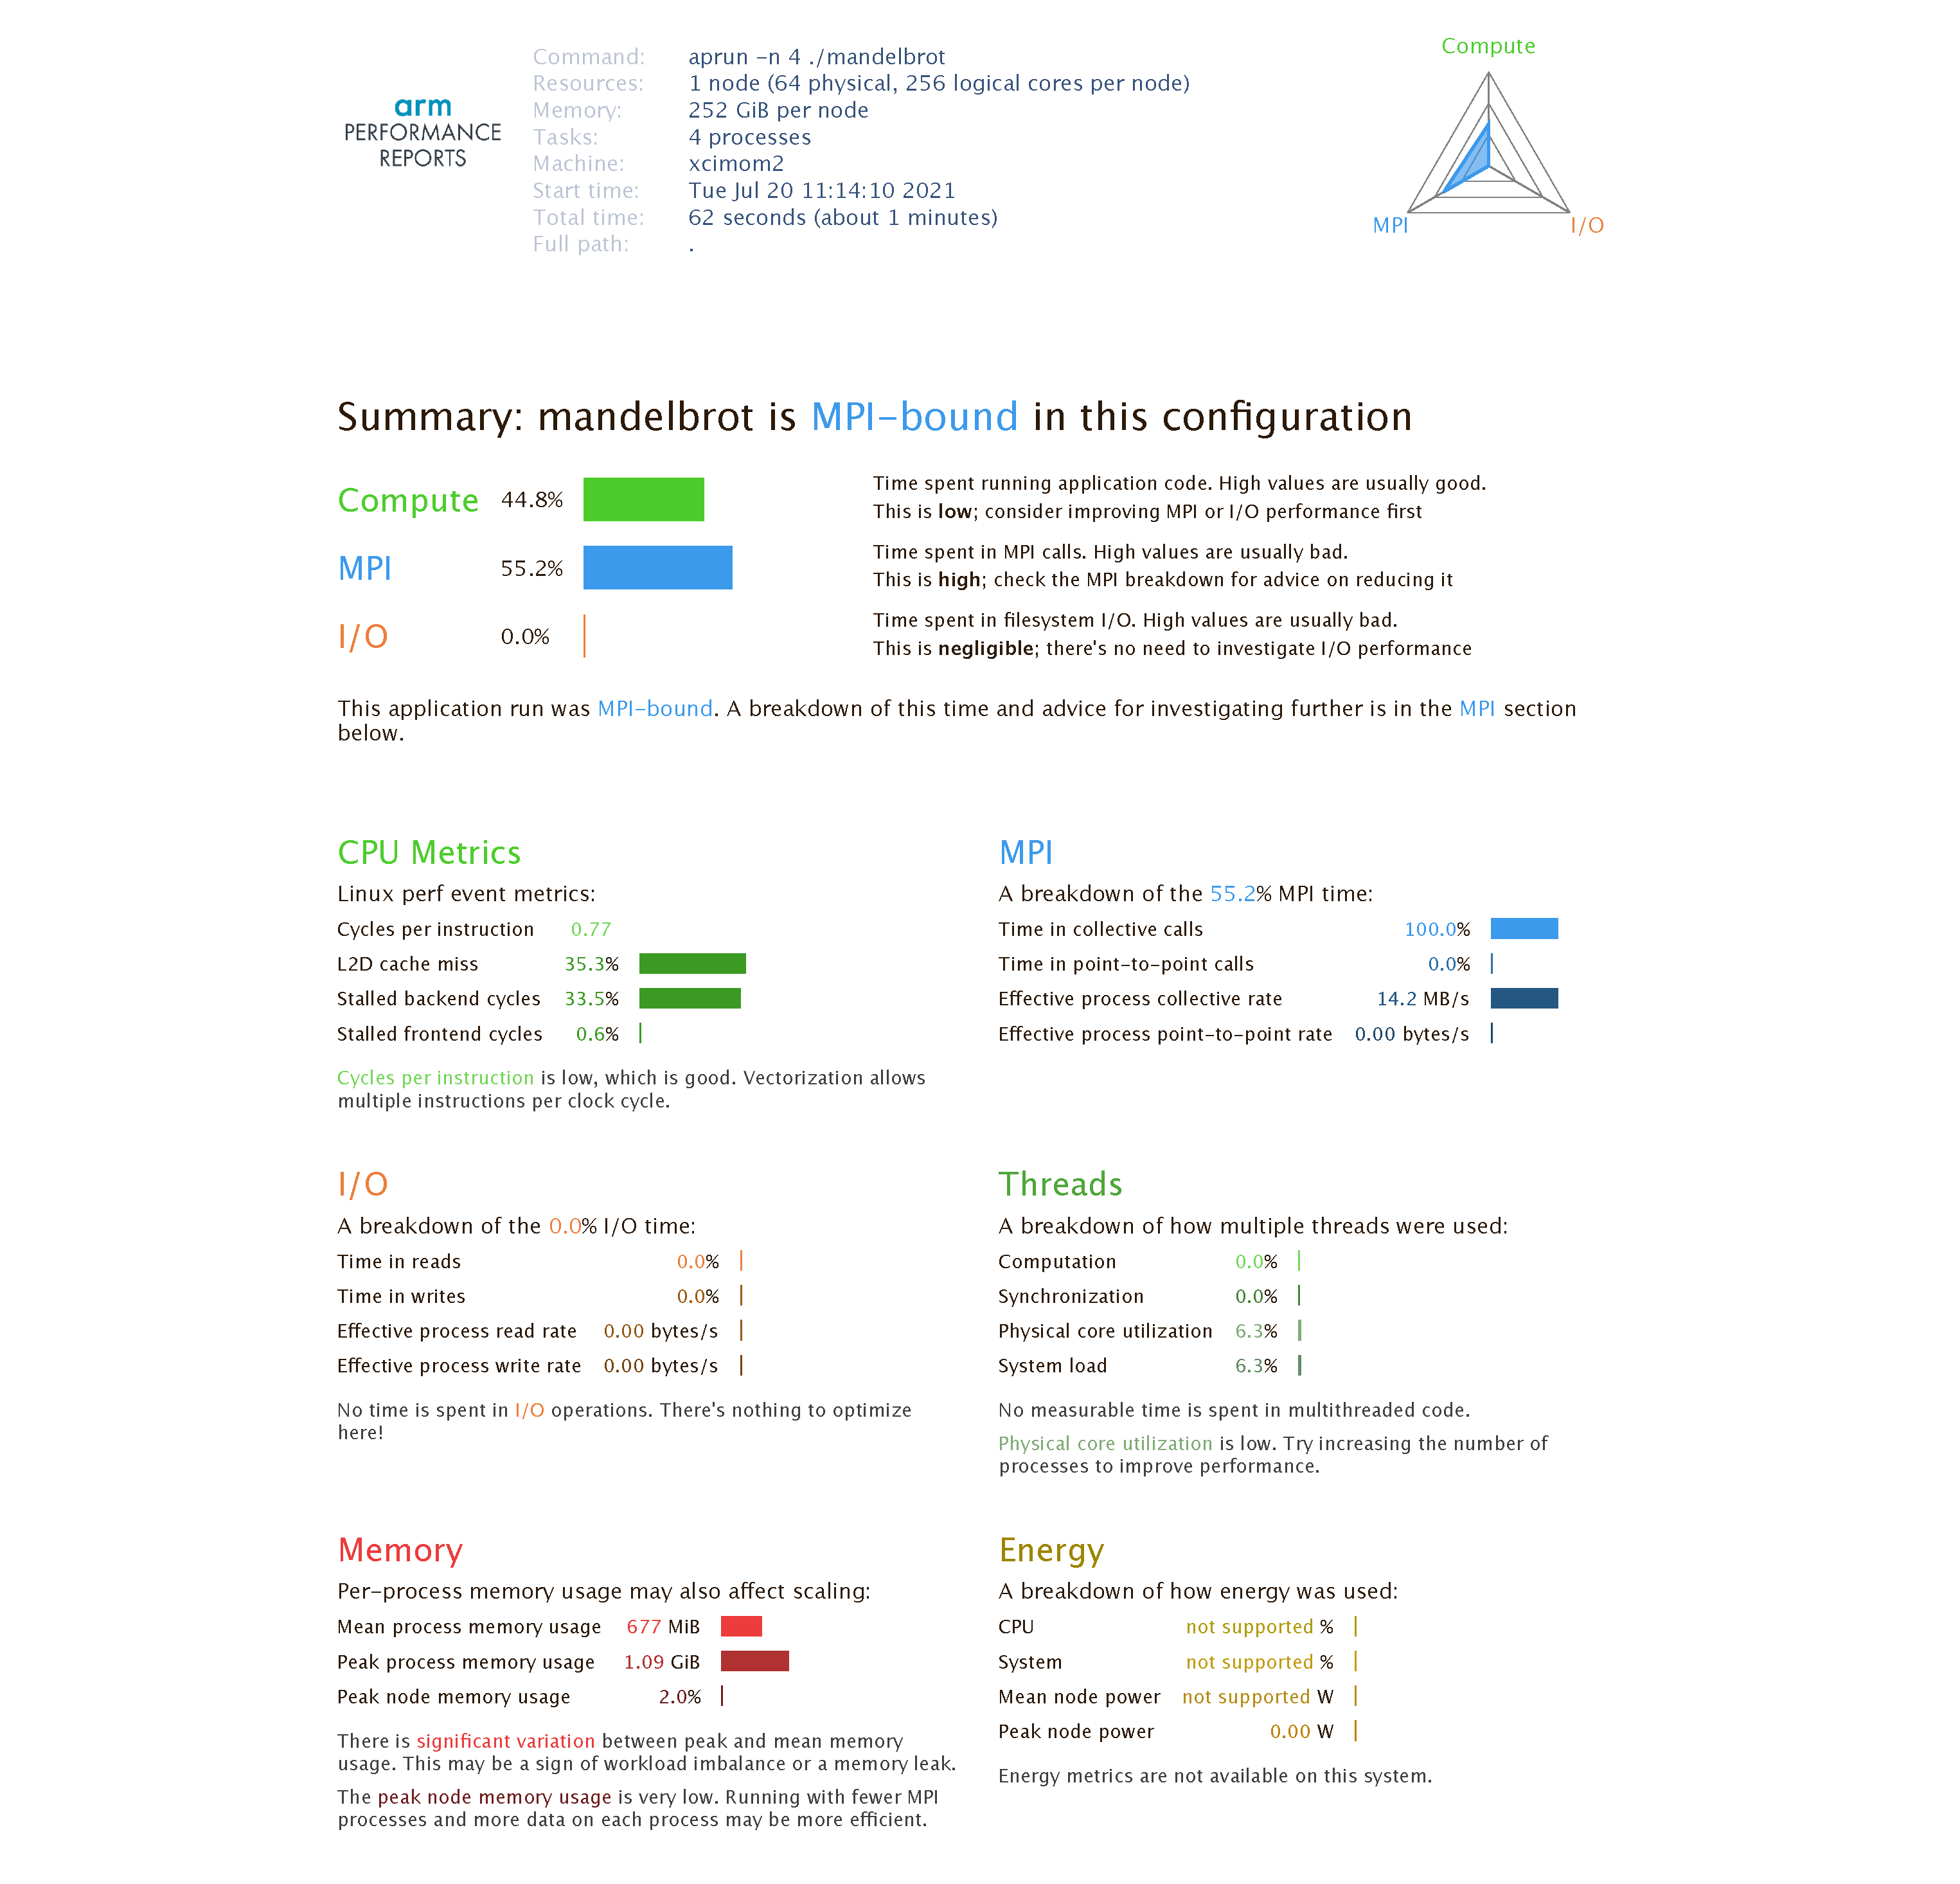
\includegraphics[scale=0.35]{figures/mandelbrot_v1_PerformanceReport}
\caption{ARM Performance Report from test 1. The tool correctly identifies that there is excessive time spent in MPI calls but does not identify load imbalance as the performance issue.}
\label{fig:perf-report_MB1}
\end{center}
\end{figure}
Performance Reports correctly identifies that the application is MPI bound but without the time line it is not clear that load imbalance is responsible.
A similar fraction of time is spent in MPI calls to that shown in the ITAC example (the corresponding ITAC output is shown in figure~\ref{fig:test1_ITAC_summary}). Performance Reports also includes summaries of other statistics, for example CPU, I/O and memory metrics. \\

\noindent
\textbf{Test 2:} results from this test are shown in figure~\ref{fig:perf-report_MB1_IO}.
\begin{figure}[htbp]
\begin{center}
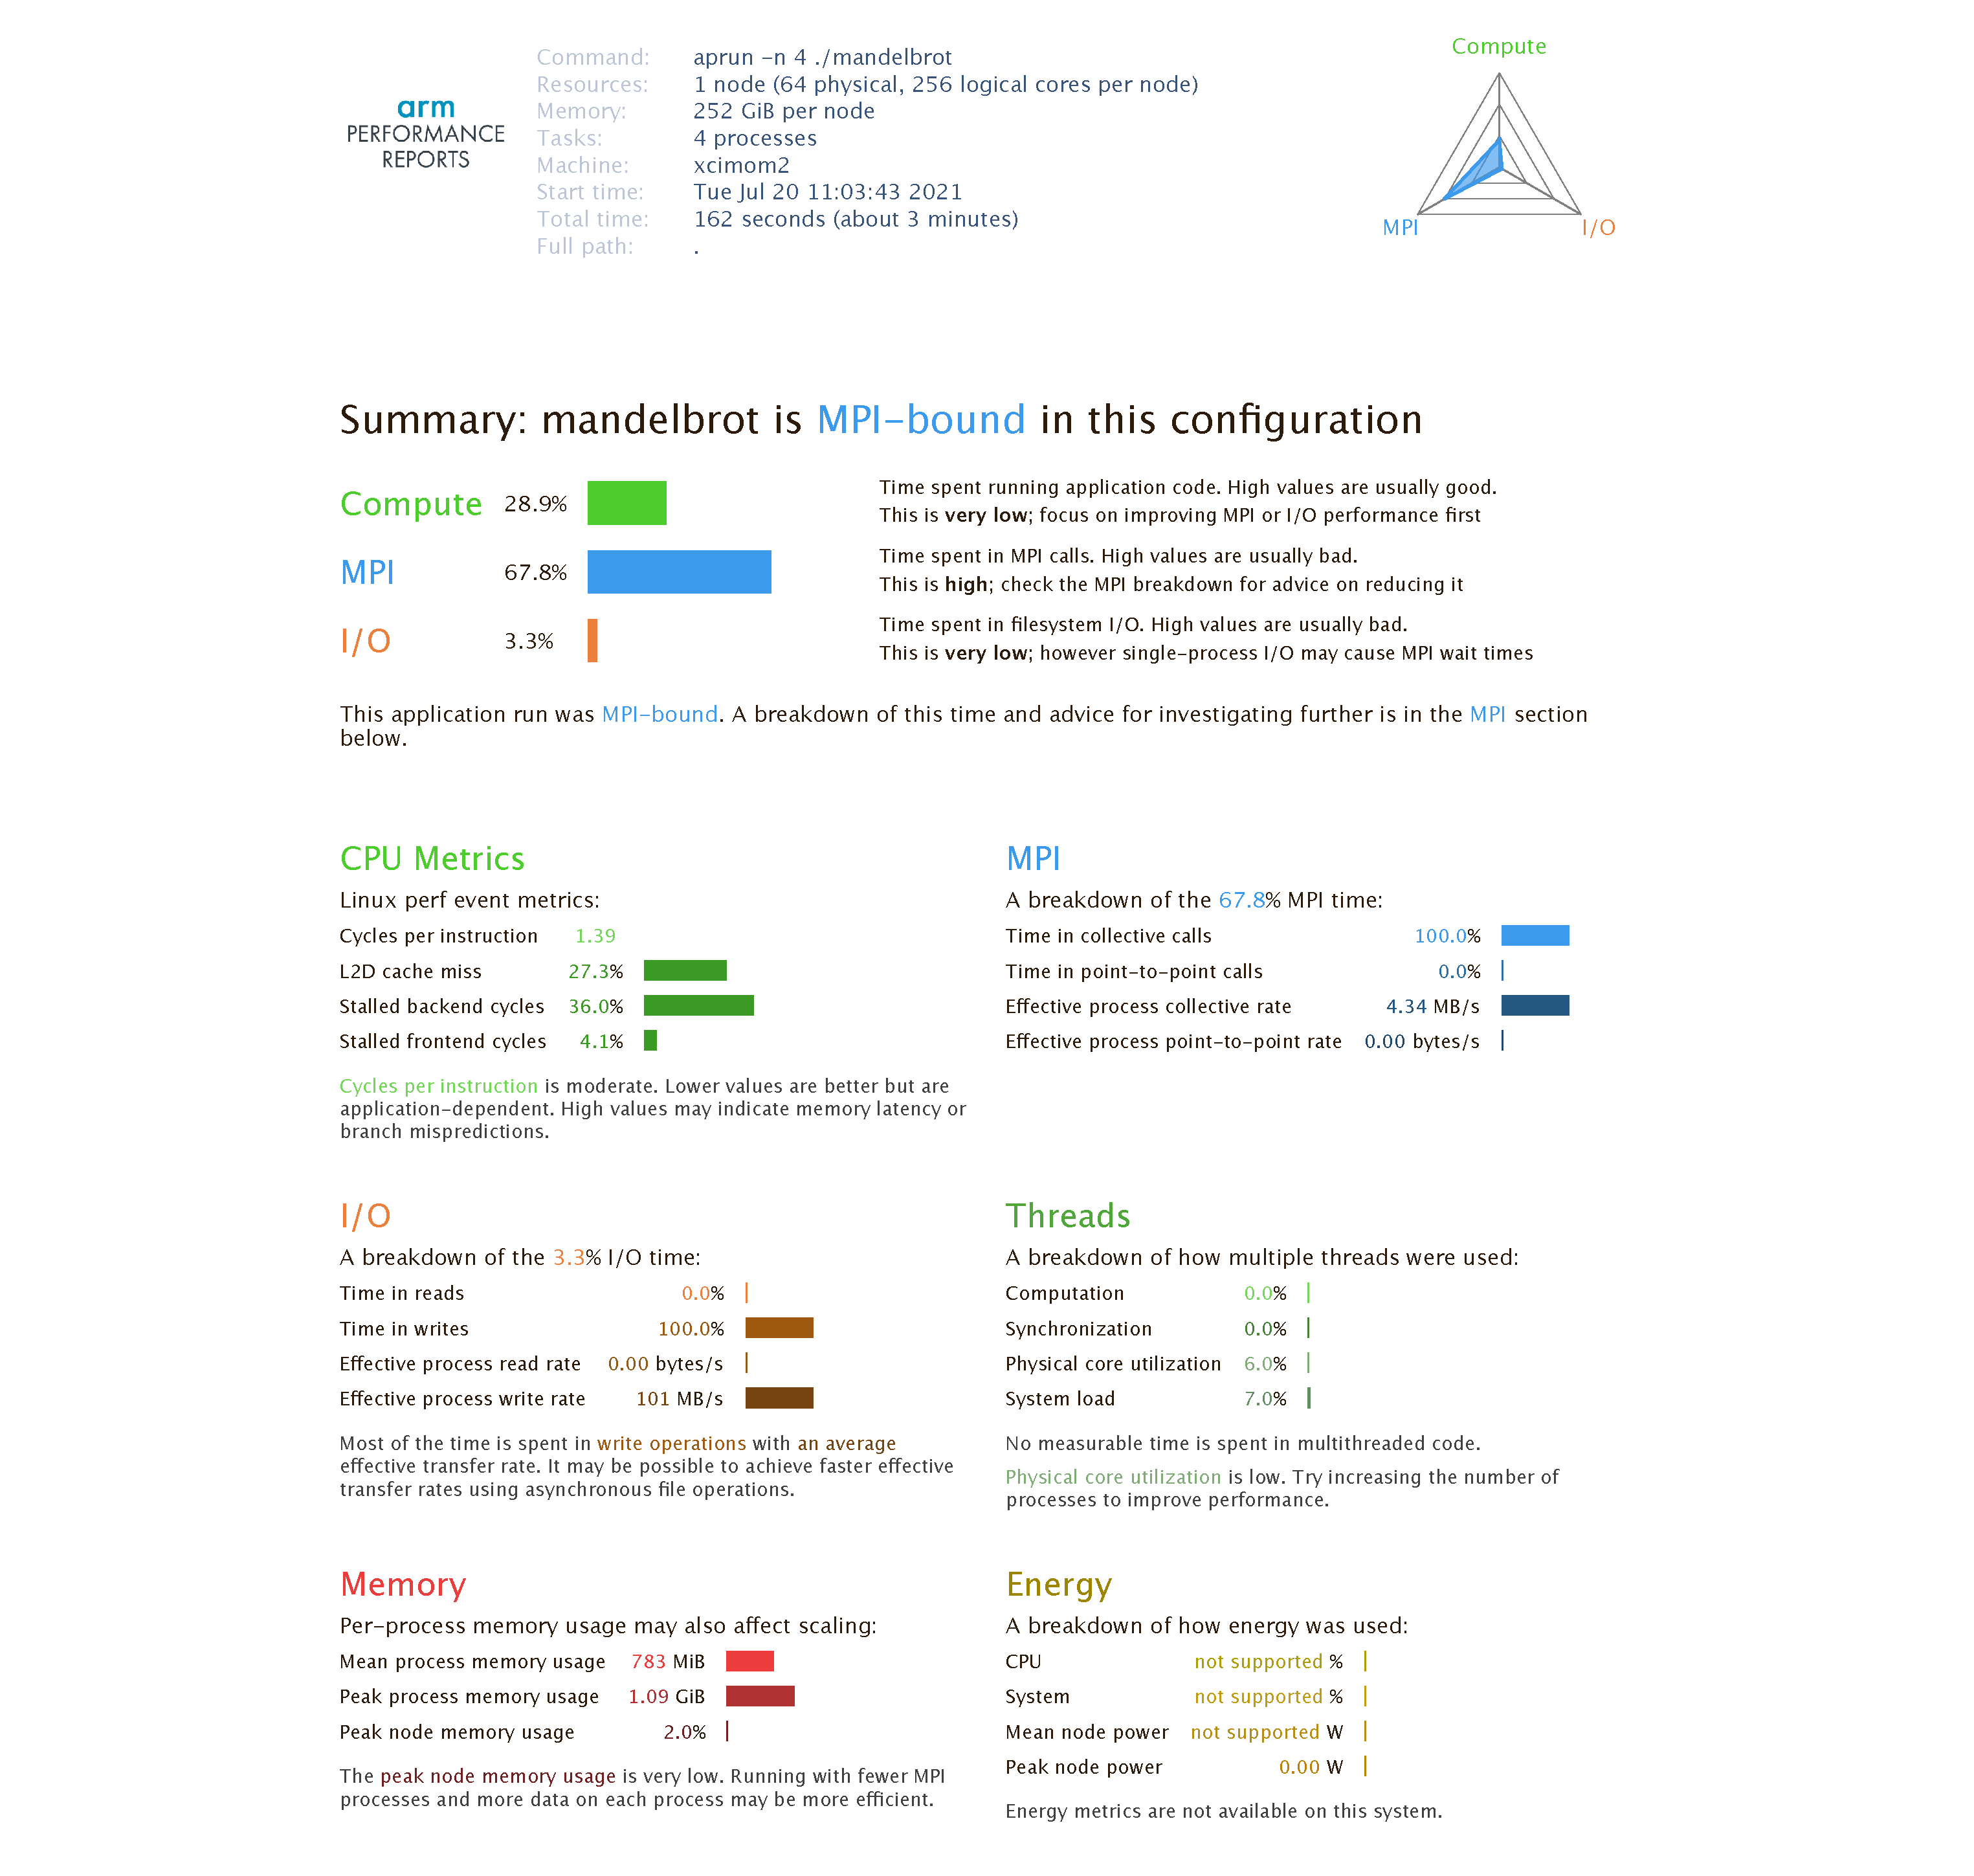
\includegraphics[scale=0.35]{figures/mandelbrot_v1_IO_PerformanceReport}
\caption{ARM Performance Report from test 2 which is like test 1 but with I/O enabled. The additional time spent in I/O causes an exacerbated load imbalance due to I/O being funnelled through the rank zero process which has increased the fraction of time spent in MPI calls. }
\label{fig:perf-report_MB1_IO}
\end{center}
\end{figure}
This test is like test 1 but with I/O enabled and time spent in I/O is now seen in the Performance Report. However the main performance issue caused by the I/O is actually 
an exacerbated load imbalance due to I/O being funnelled through the rank zero process causing all other processes to wait at an MPI barrier. Although slow I/O is the underlying cause the time spent in I/O is only a small fraction of the time breakdown and the main impact is additional time spend in MPI collectives. \\

\noindent
\textbf{Test 3:} results from this test are shown in ~\ref{fig:perf-report_test3}
\begin{figure}[htbp]
\begin{center}
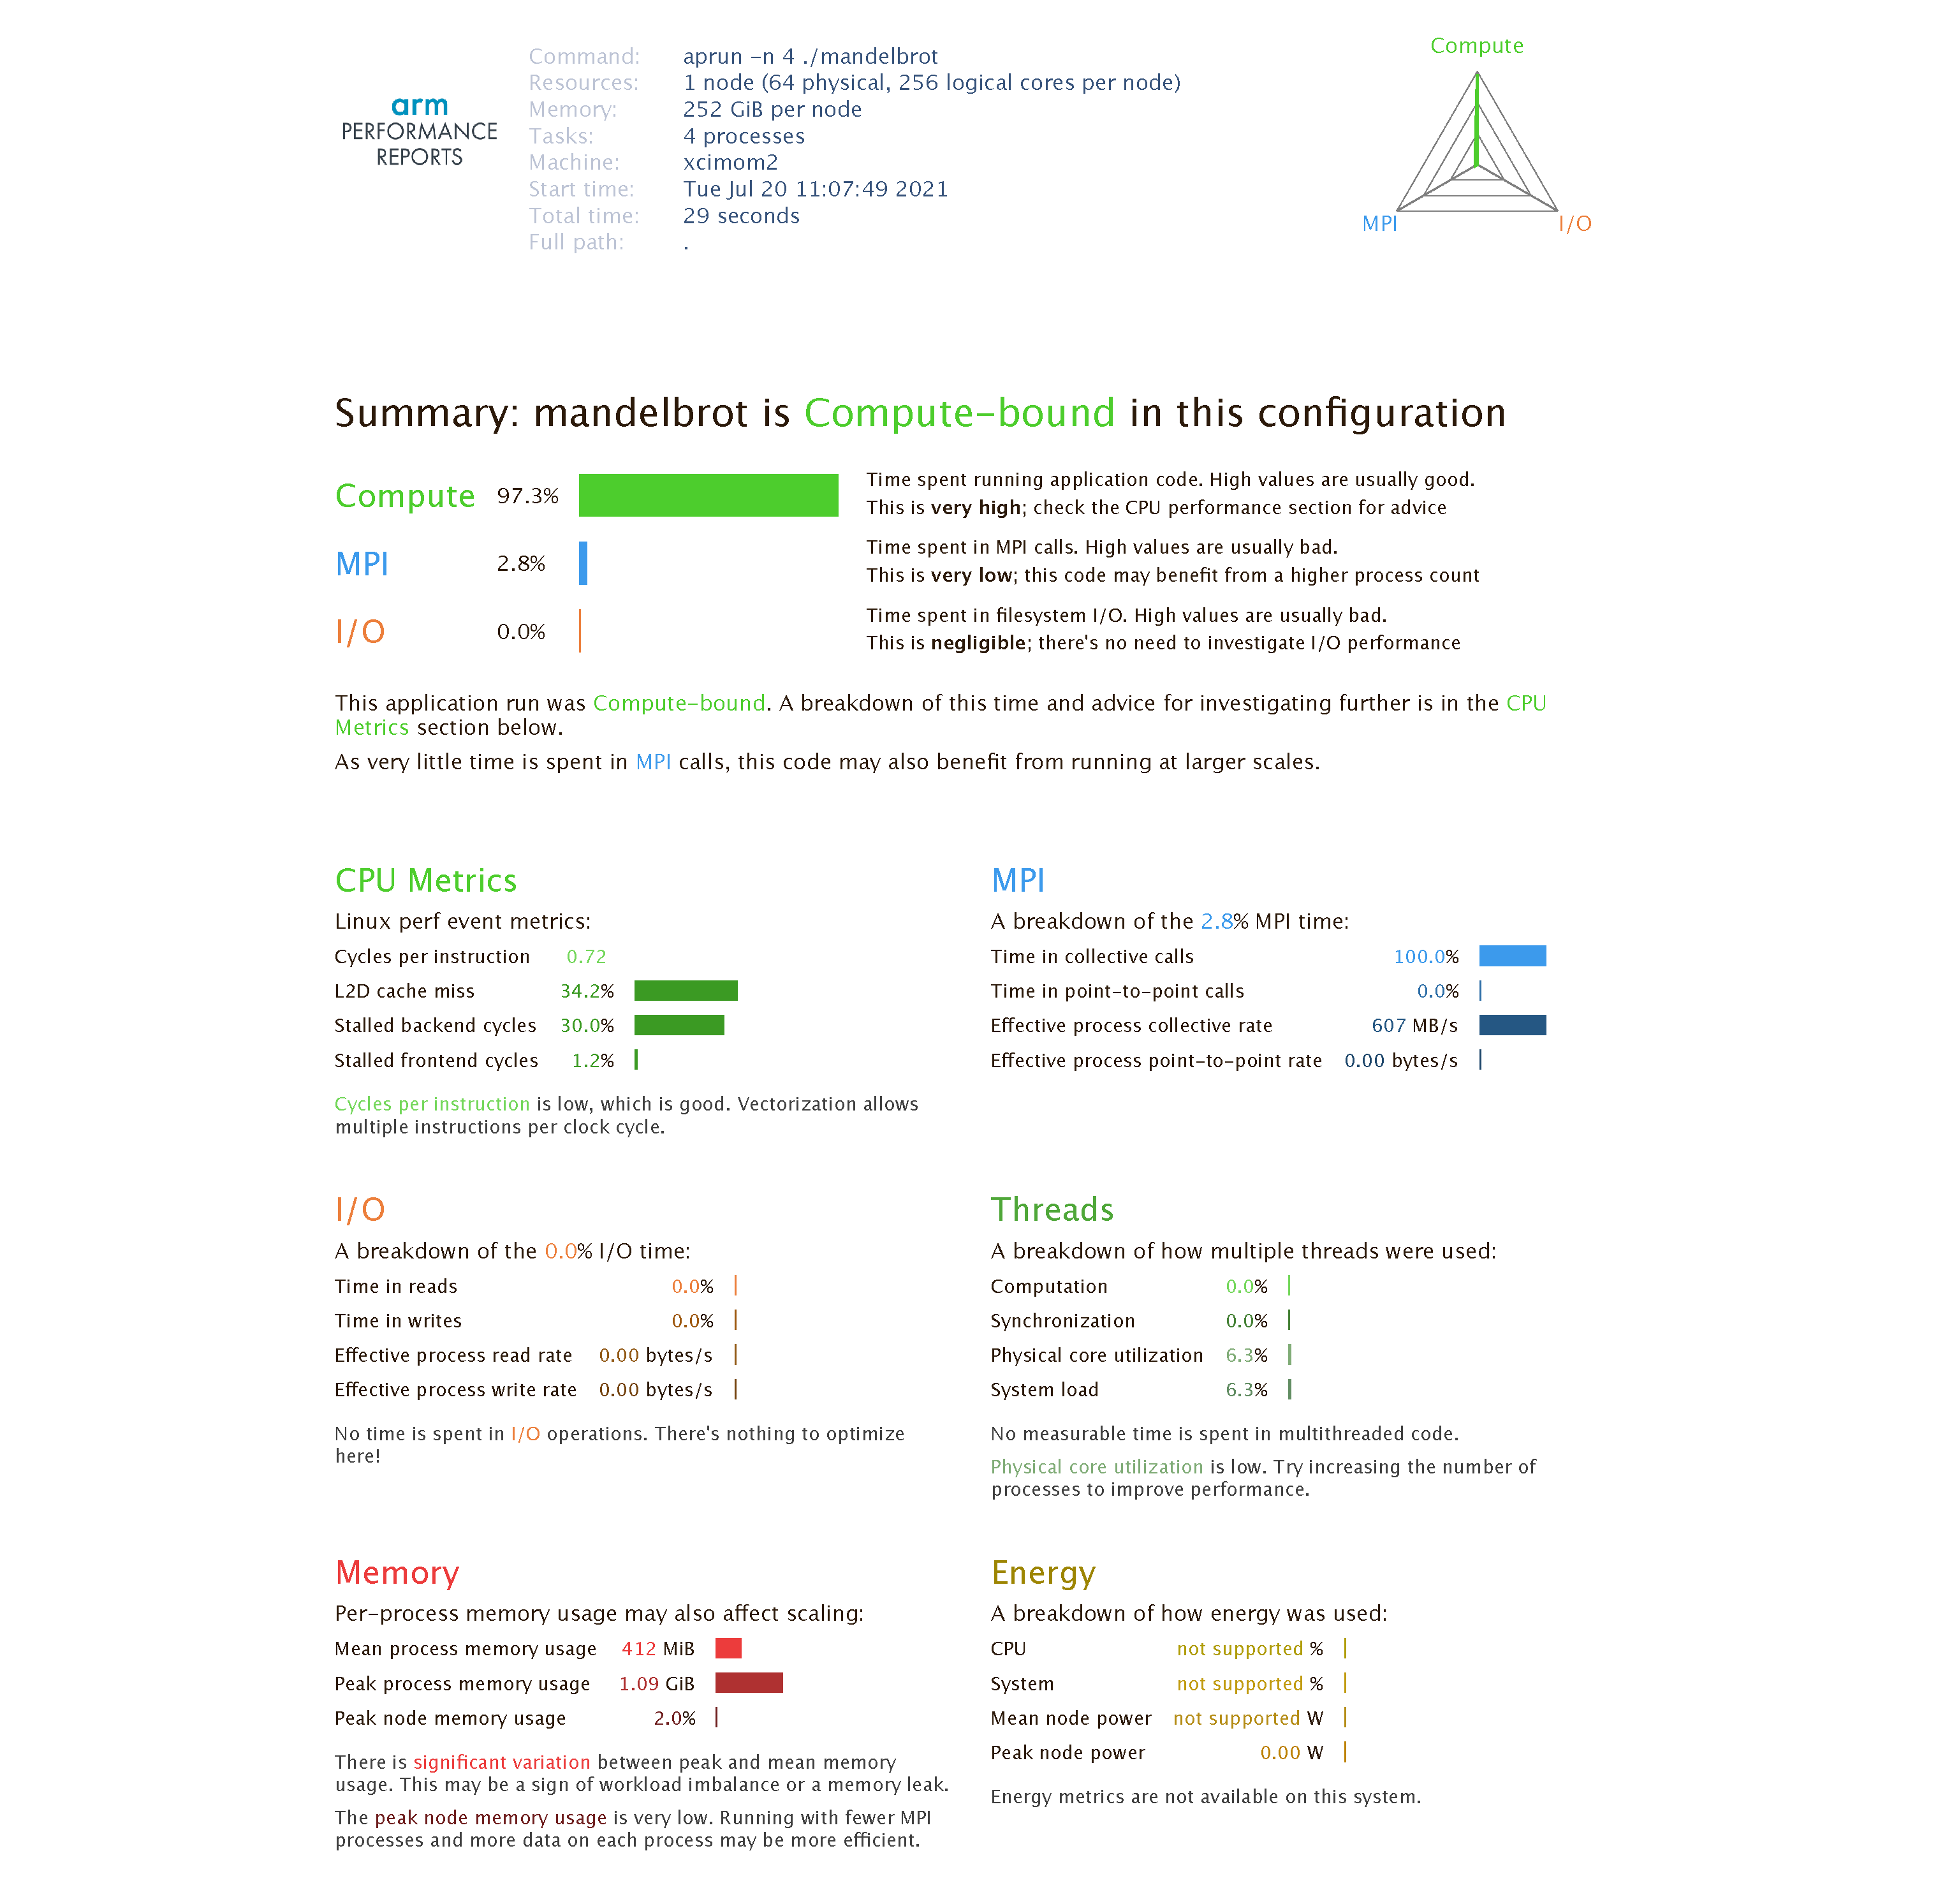
\includegraphics[scale=0.35]{figures/mandelbrot_v2_PerformanceReport}
\caption{ARM Performance Report from test 3. This version has fixed the load imbalance by interleaving iterations on the real axis.}
\label{fig:perf-report_test3}
\end{center}
\end{figure}
The fraction of time spent in MPI is now low (around 2\%) as the load imbalance has been corrected. The Performance Report now directs the reader to the CPU metrics section 
as the calculation is considered compute bound. \\

\noindent
\textbf{Test 4:} Figure~\ref{fig:perf-report_MB3} shows the Performance Report from test 4 (manager-worker with 4 MPI processes).
\begin{figure}[htbp]
\begin{center}
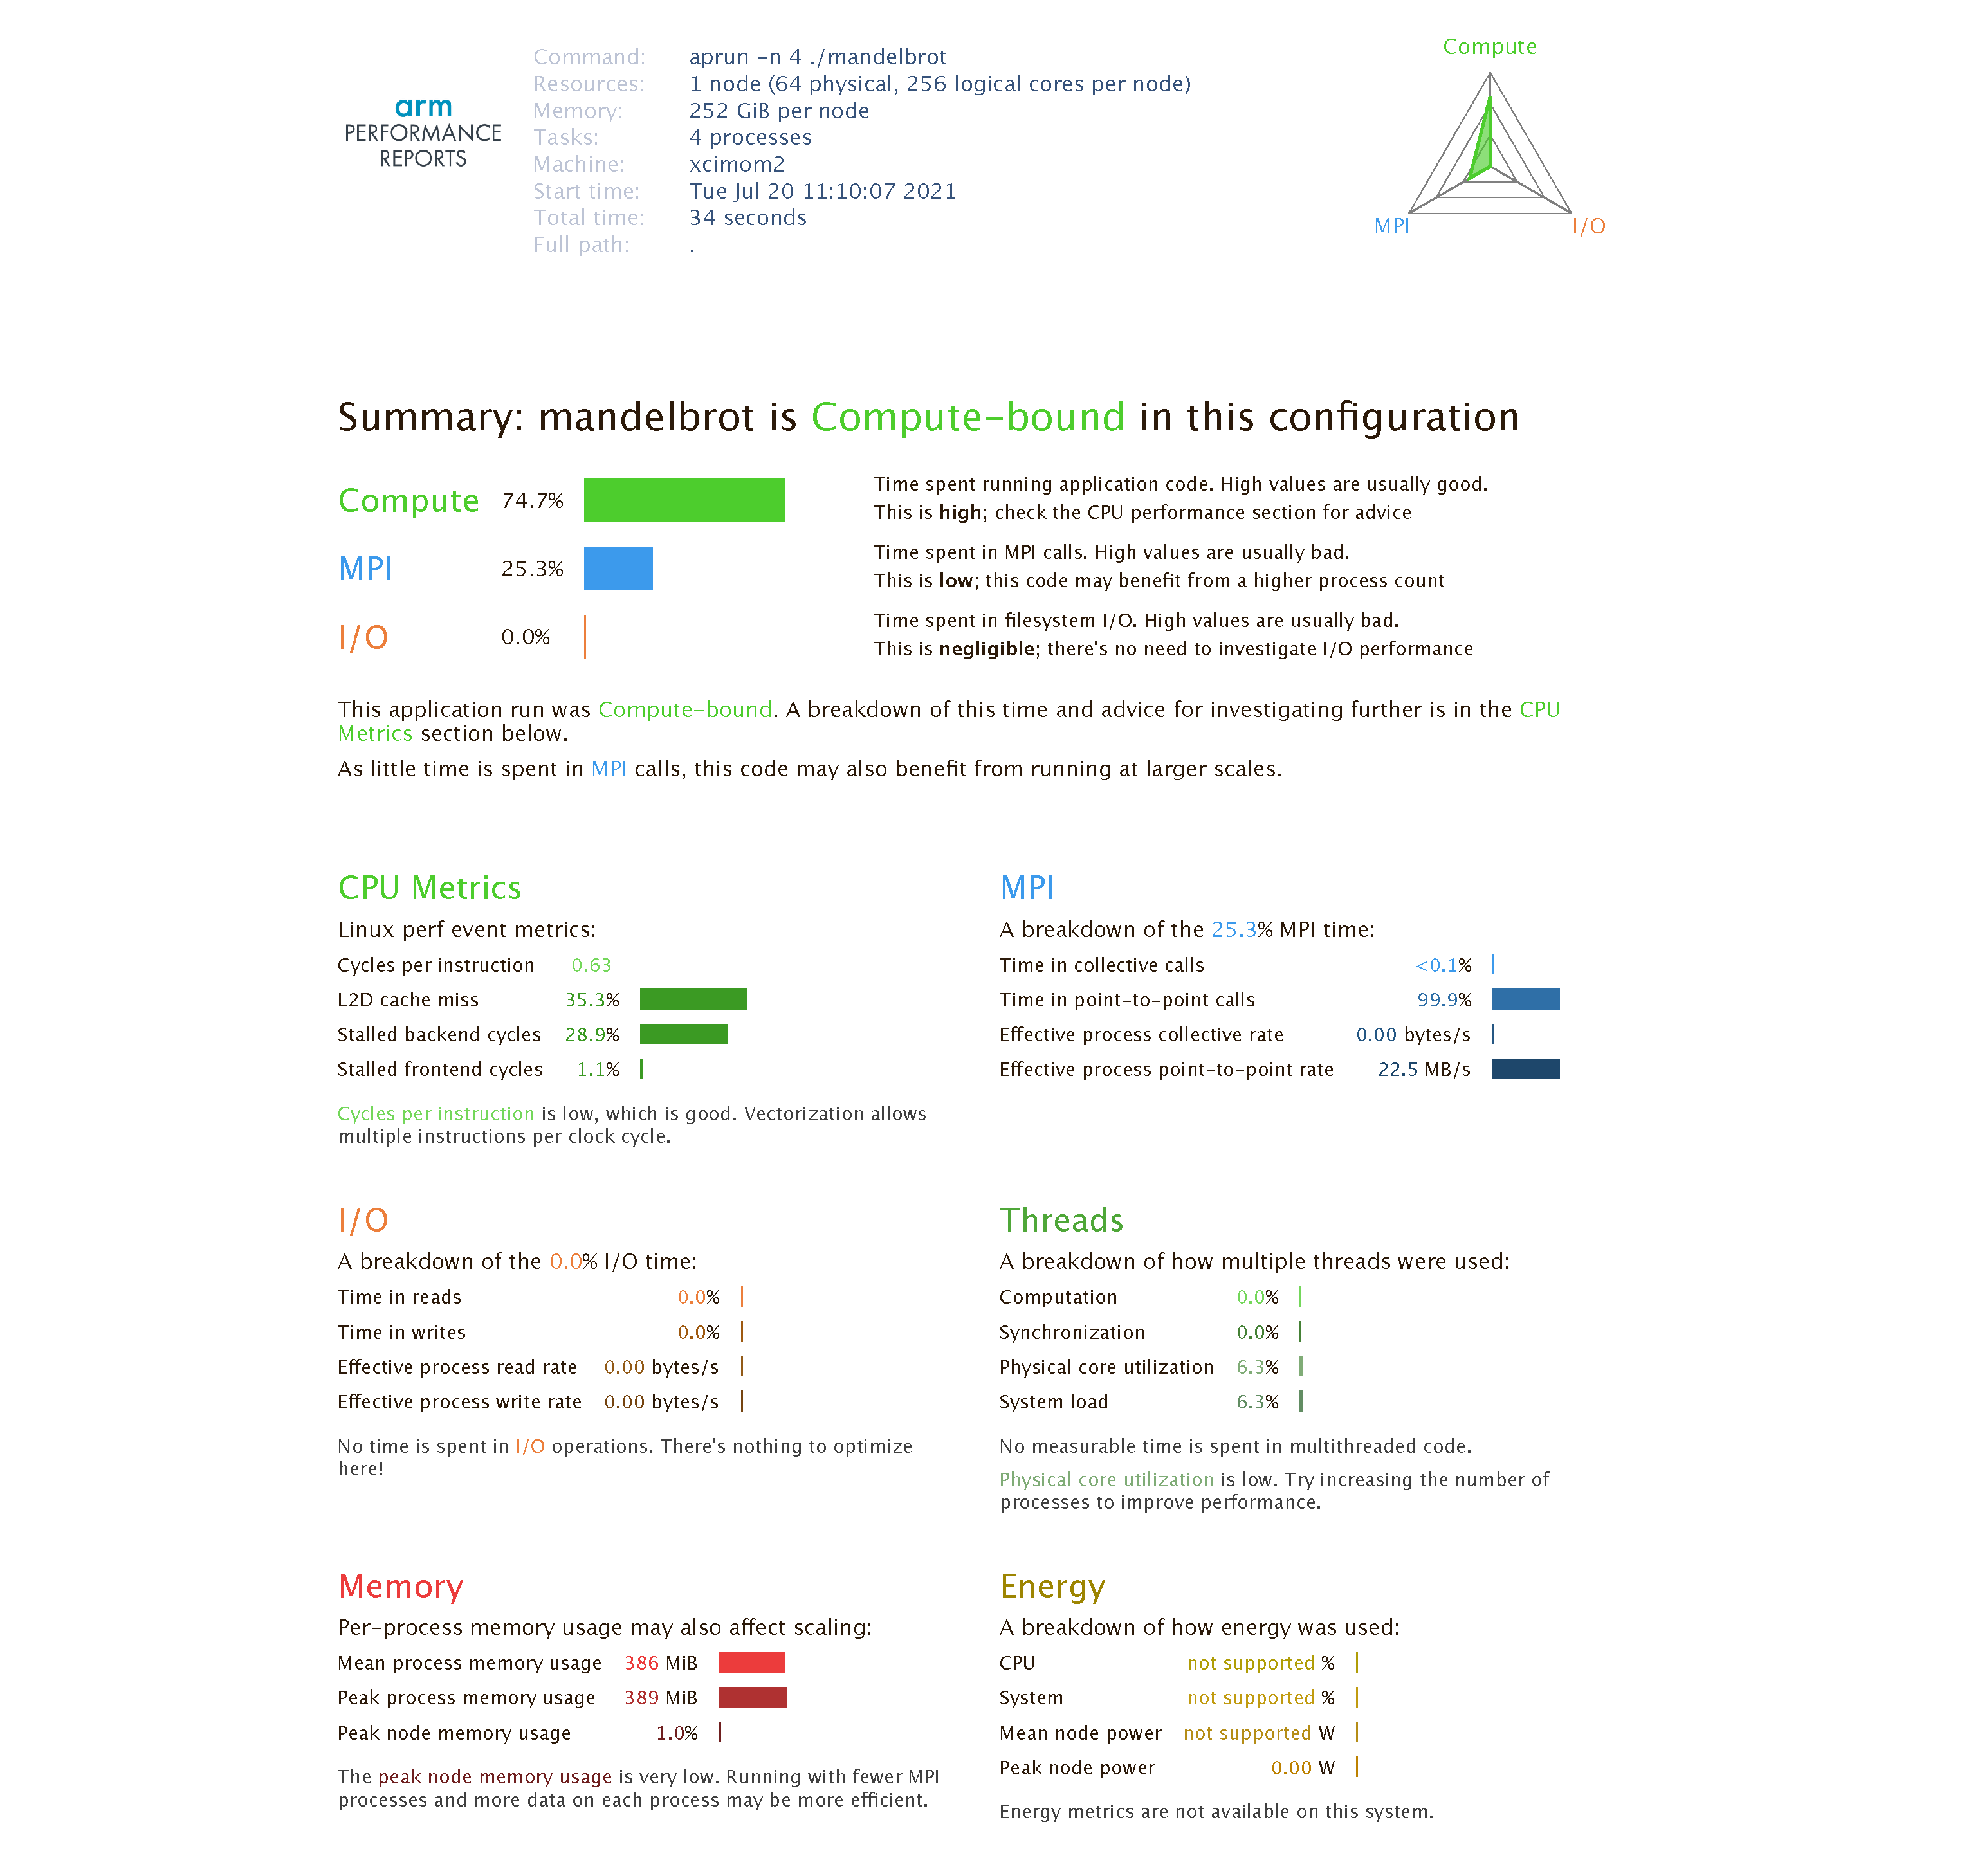
\includegraphics[scale=0.35]{figures/mandelbrot_v3_PerformanceReport}
\caption{ARM Performance Report from test 4. In the manager-worker pattern only 3 out of 4 MPI processes carry out the calculation and the fourth process is the manager which does not compute any points.}
\label{fig:perf-report_MB3}
\end{center}
\end{figure}
With this test only 3 out of 4 MPI processes carry out the calculation and the fourth process is the manager which does not compute any points. The MPI time of 25\% is consistent with the manager process waiting for results from the worker processes. In the MPI section of the Performance Report we see that almost all time is spent in point-to-point calls instead of collectives, as expected. We also see a reduction in the peak memory usage as there is no need to populate a large buffer for carrying out communication. \\

\noindent
\textbf{Test 5:} in this test the number of MPI processes is increased to 16 (see figure~\ref{fig:perf-report_MB3_16procs}) and the fraction of MPI time decreases as there are now 15 out of 16 processes actively working on the calculation instead of 3 out of 4.
\begin{figure}[htbp]
\begin{center}
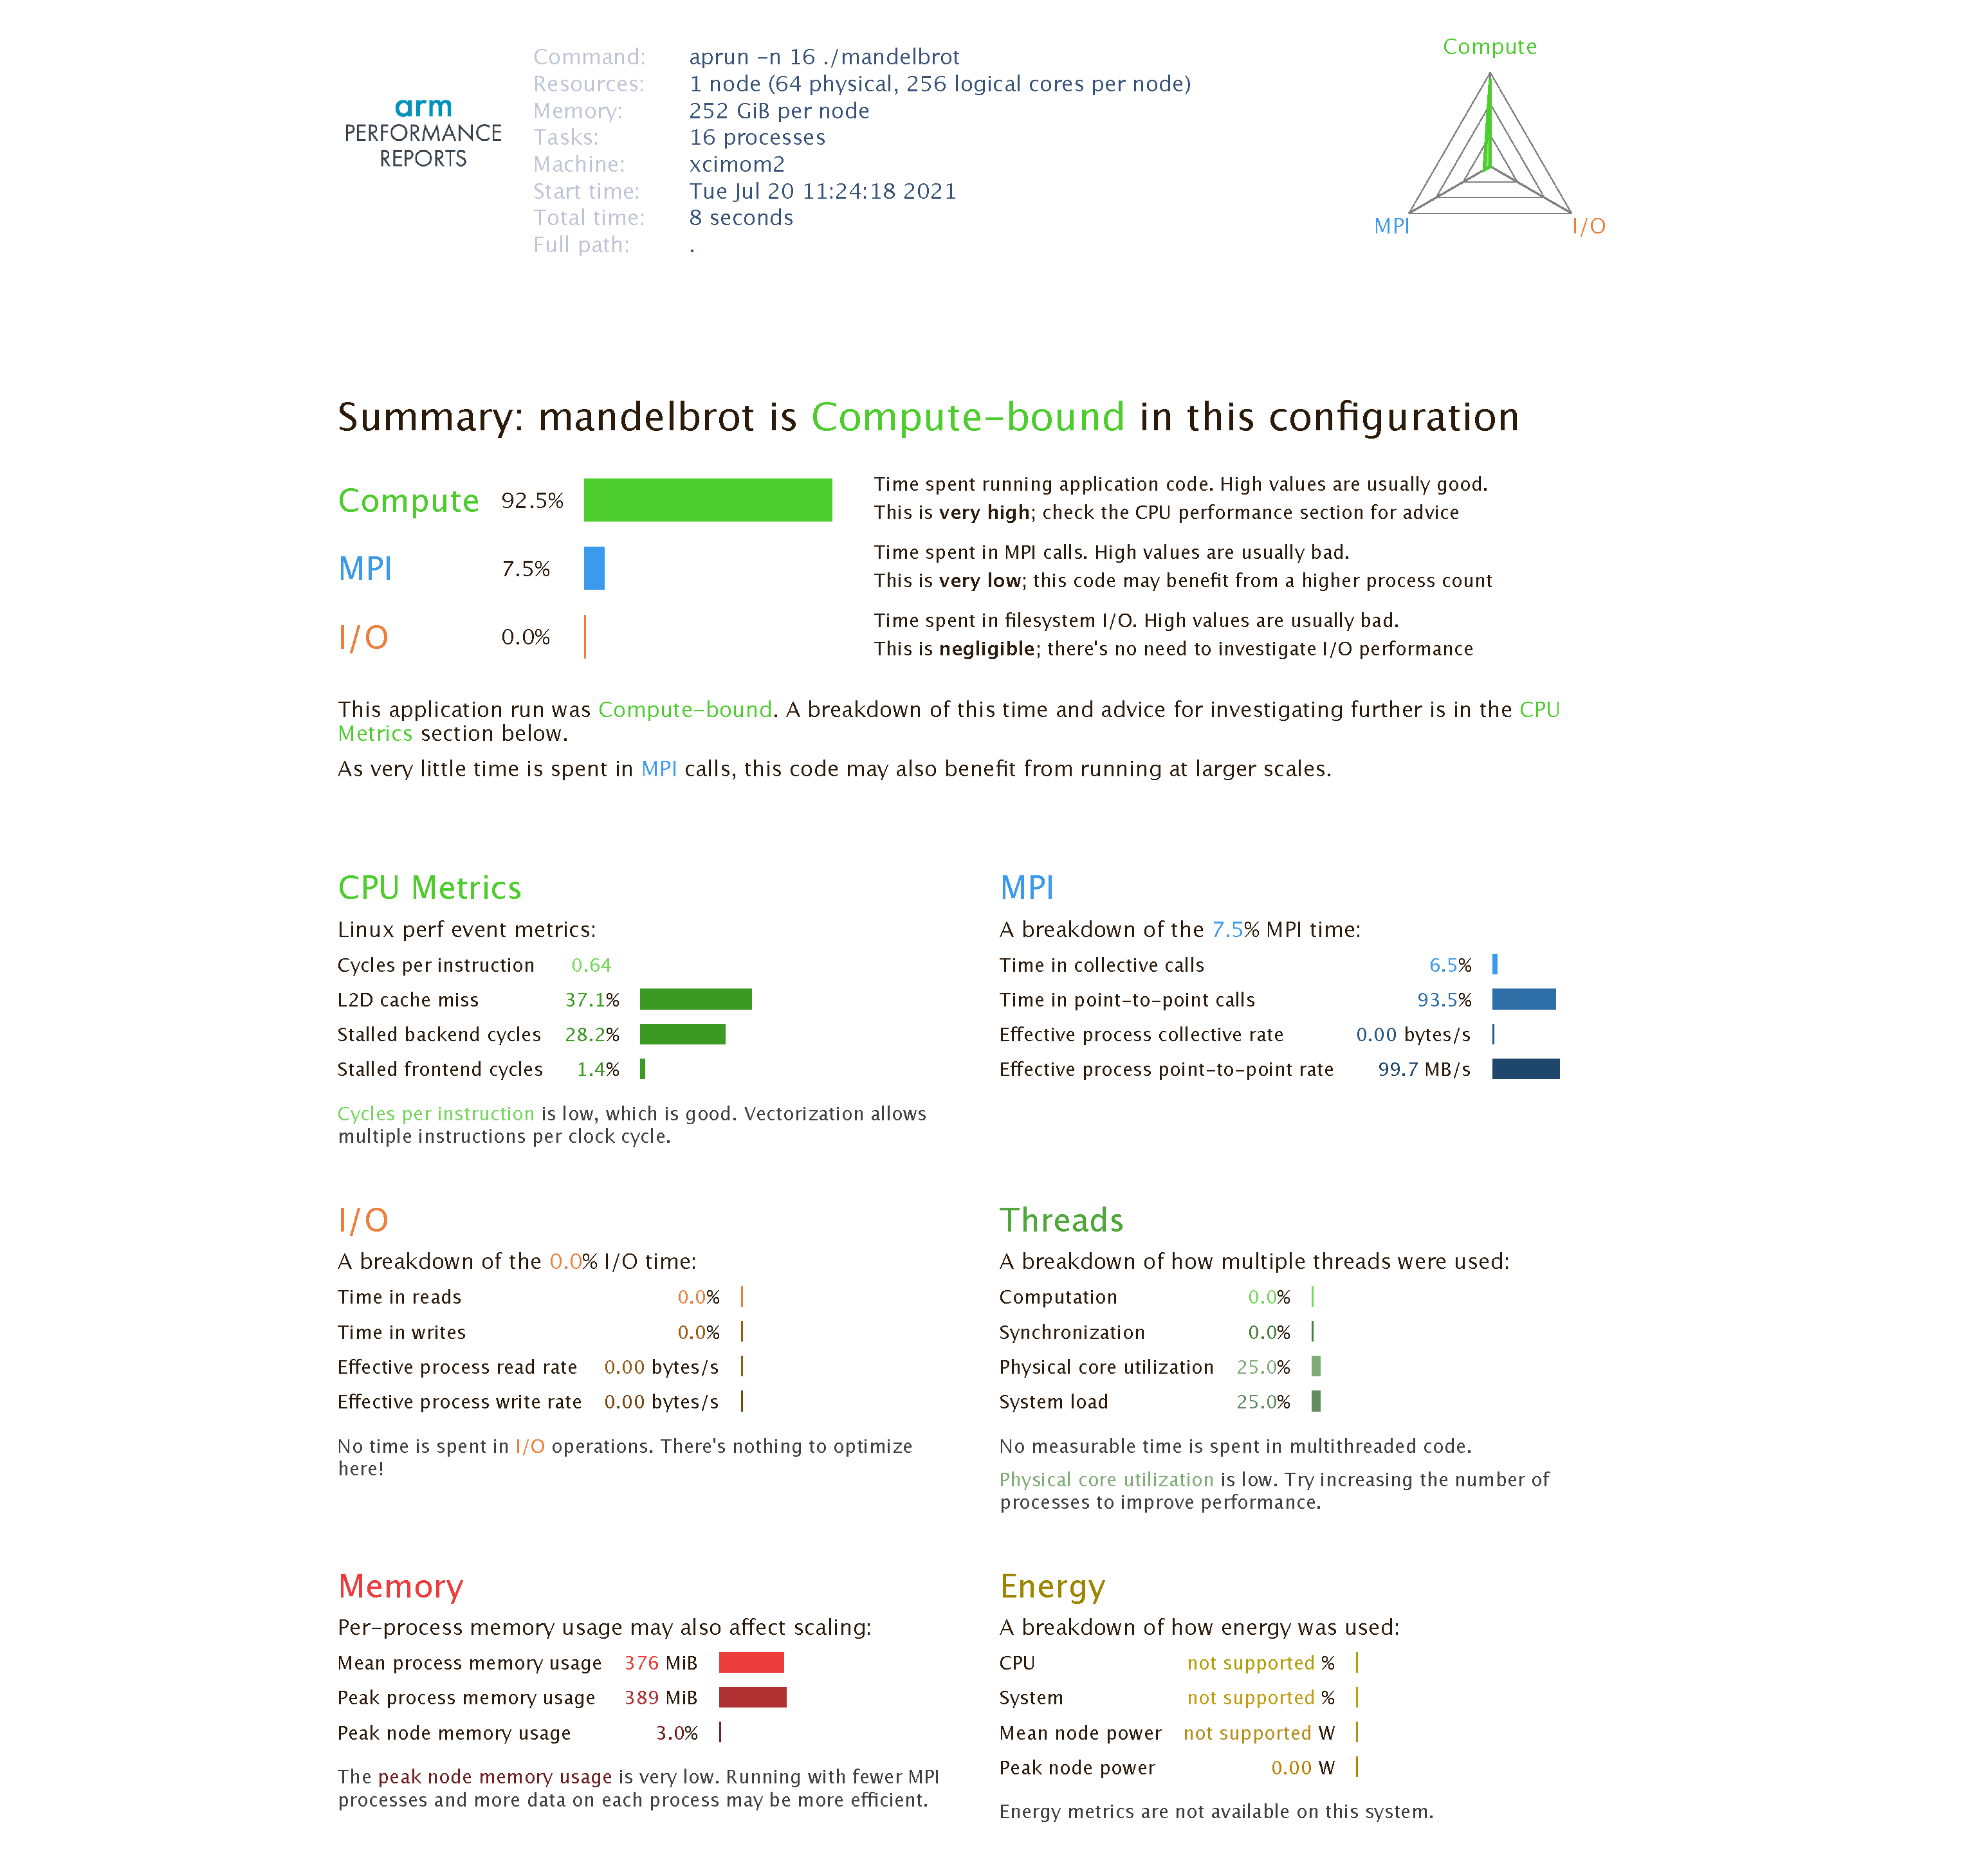
\includegraphics[scale=0.35]{figures/mandelbrot_v3_16procs_PerformanceReport}
\caption{ARM Performance Report from test 5. This test uses the manager-worker version of the program (like test 4) but with 16 processes instead of 4. The MPI fraction is now reduced as the manager process is only one out of sixteen processes instead of one out of three.}
\label{fig:perf-report_MB3_16procs}
\end{center}
\end{figure}

\subsubsection{MAP}

MAP provides more comprehensive information than Performance Reports and if the application is compiled with a \verb+-g+ flag then function-level information can be obtained (although this is not required for MAP to work). When profiling an application with MAP modify the job script to load the Forge module (as for performance reports) and modify the aprun command by prepending \verb+map --profile+ e.g. replace
\begin{verbatim}
aprun -n ${nprocs} ./mandelbrot
\end{verbatim}
with
\begin{verbatim}
map --profile aprun -n ${nprocs} ./mandelbrot
\end{verbatim}
When the application runs a file with a \verb+.map+ extension is generated which can be loaded into the map graphical interface:
\begin{verbatim}
> module load tools/arm-forge
> map mandelbrot_4p_1n_1t_2021-08-05_17-23.map &
\end{verbatim}

Example output from two of the tests (tests 1 and 5) will to shown to demonstrate the MAP tool. Output from profiling test 1 with MAP is shown in figure~\ref{fig:MAP_test1}.
%
\begin{figure}[htbp]
\begin{center}
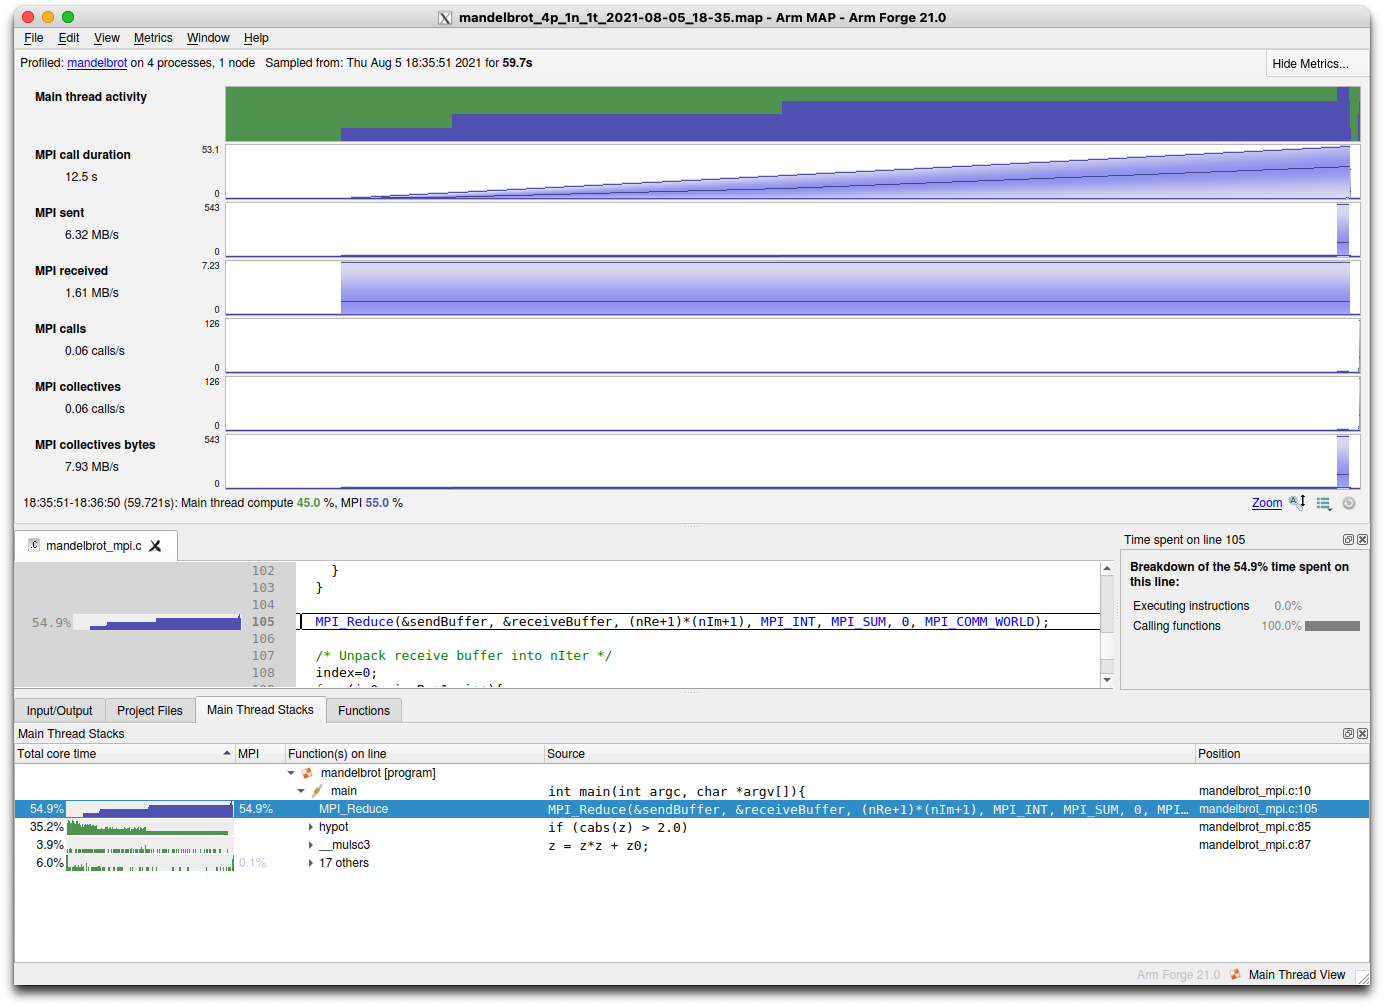
\includegraphics[scale=0.3]{figures/MAP_test1}
\caption{Results from profiling test 1 using MAP. The ``Main thread activity'' panel shows the load imbalance and
we can see the specific line which calls the \texttt{MPI\_Reduce} as the executable has been compiled with a \texttt{-g} flag.}
\label{fig:MAP_test1}
\end{center}
\end{figure}
This view was set up by selecting \texttt{Metrics} $\rightarrow$ \texttt{Preset: MPI} to load the preset view of MPI events. The point-to-point metrics were then switched off (under the \texttt{Metrics} menu) as there are no point-to-point calls in this particular example. The ``Main thread activity'' panel shows the load imbalance. The green bars show application activity and these complete at different times and the MPI call duration ramps up as processes reach the \verb+MPI_Reduce+ and are forced to wait\footnote{See \url{https://developer.arm.com/documentation/101136/2103/MAP/Metrics-view/MPI-calls} for more information on interpreting MAP MPI plots}. The executable has been compiled with a \texttt{-g} flag, which enables mapping back to line numbers on the source code, and in the middle panel we see the line number where the \verb+MPI_Reduce+ is called. 

Output from profiling test 5 is shown in figure~\ref{fig:MAP_test5} (this time all the MPI metrics have been left switched on).
\begin{figure}[htbp]
\begin{center}
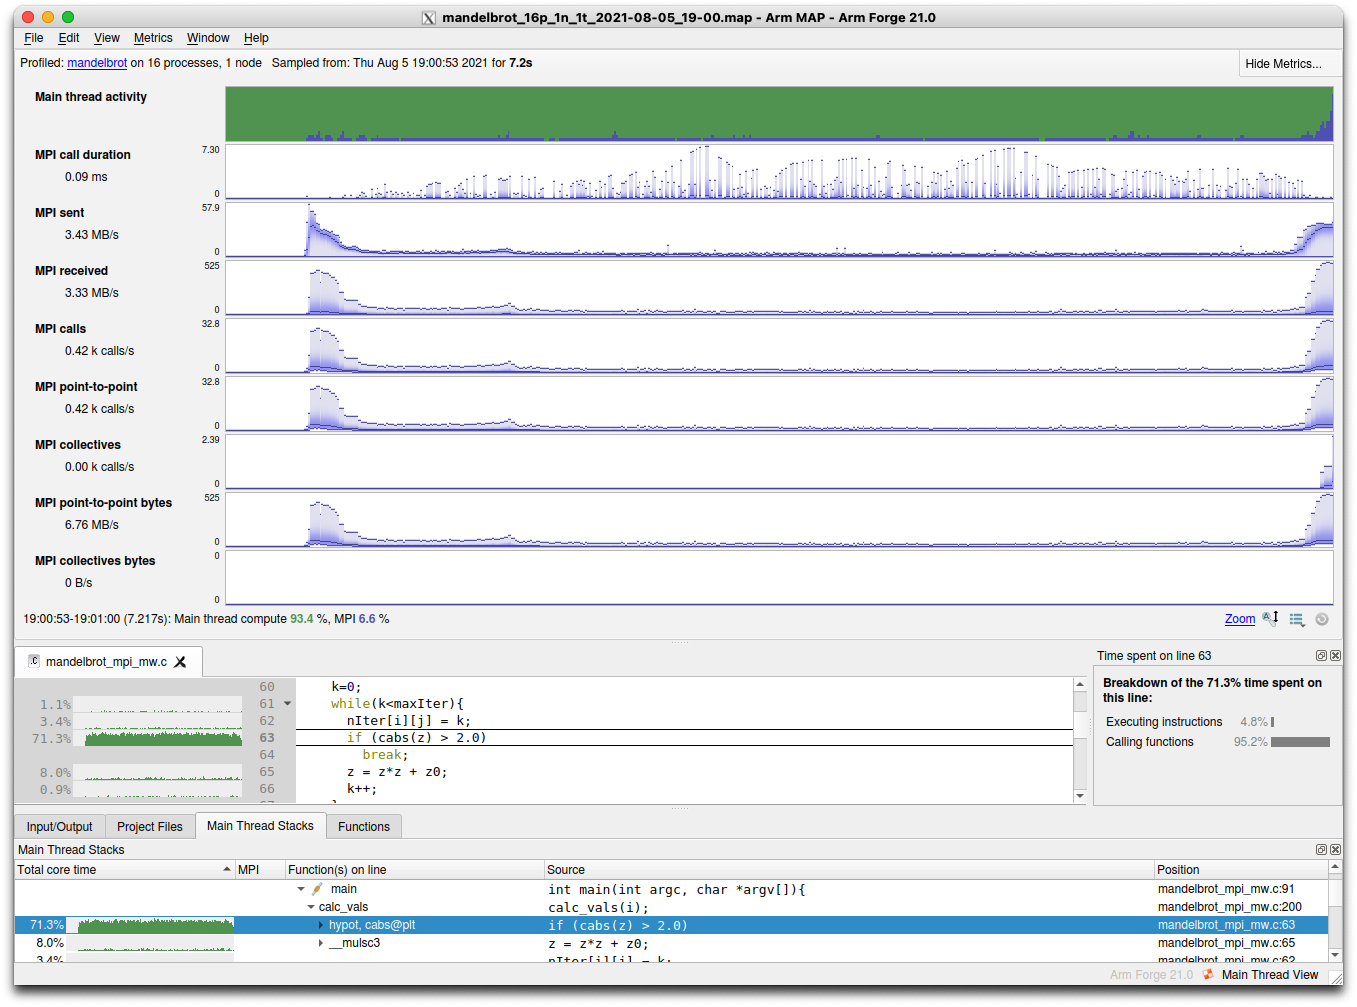
\includegraphics[scale=0.3]{figures/MAP_test5}
\caption{Results from profiling test 5 using MAP. This is a manager-worker pattern which carries out a large number of point-to-point communications.}
\label{fig:MAP_test5}
\end{center}
\end{figure}
The MPI sent and MPI received time lines show the number of bytes per second passed to MPI send and receive functions respectively. These plots show higher levels of activity at the beginning and end of the calculation when the workers are completing work units more rapidly. At the end of the application we see some time spent in a collective which transfers no data and this is the \verb+MPI\_Barrier+ at the end of the program.

\pagebreak

%---------------------------------------------------------------------------------------------------------------------

\subsection{Cray PAT}

Cray PAT (Performance Analysis Tools) is a suite of profiling tools which are available on Cray systems. Cray PAT has a large number of features\footnote{See \url{https://docs.nersc.gov/tools/performance/craypat/}} but also has a simplified mode called \verb+perftools-lite+. In section tests 1 and 5 will be run using \verb+perftools-lite+ to demonstrate this mode of operation. 

To enable profiling with \verb+perftools-lite+ the \verb+perftools-lite+ module is loaded and the executable compiled using as usual. For example to build with the GCC compiler and profiling:
\begin{verbatim}
> module switch PrgEnv-cray PrgEnv-gnu 
> module load perftools-lite
> cc -o mandelbrot mandelbrot_mpi.c 
WARNING: PerfTools is saving object files from a temporary directory into directory 
'/home/username/.craypat/mandelbrot/178976'
INFO: creating the PerfTools-instrumented executable 'mandelbrot' (lite-samples) ...OK
\end{verbatim}
When the \verb+cc+ wrapper script is run it reports that that PerfTools is instrumenting the executable as expected.
The job can then be submitted to the queue using an unmodified job script (the \texttt{perftool-base} module is loaded as part of the programming environment and does not need to be explicitly loaded in the job script). When the job runs profiling information is written into a new directory (e.g. \verb+mandelbrot+10863-42s+) with a summary written to the stdout file (see Appendix A for example output). There is a graphical interface called ``Apprentice 2'' which can be used to view the output in the profiling directory e.g. 
\begin{verbatim}
> app2 mandelbrot+10863-42s &
\end{verbatim}

Figure~\ref{fig:app2_summary} shows the Apprentice 2 overview window from \texttt{pertools-lite} profiling of test 1. 
\begin{figure}[htbp]
\begin{center}
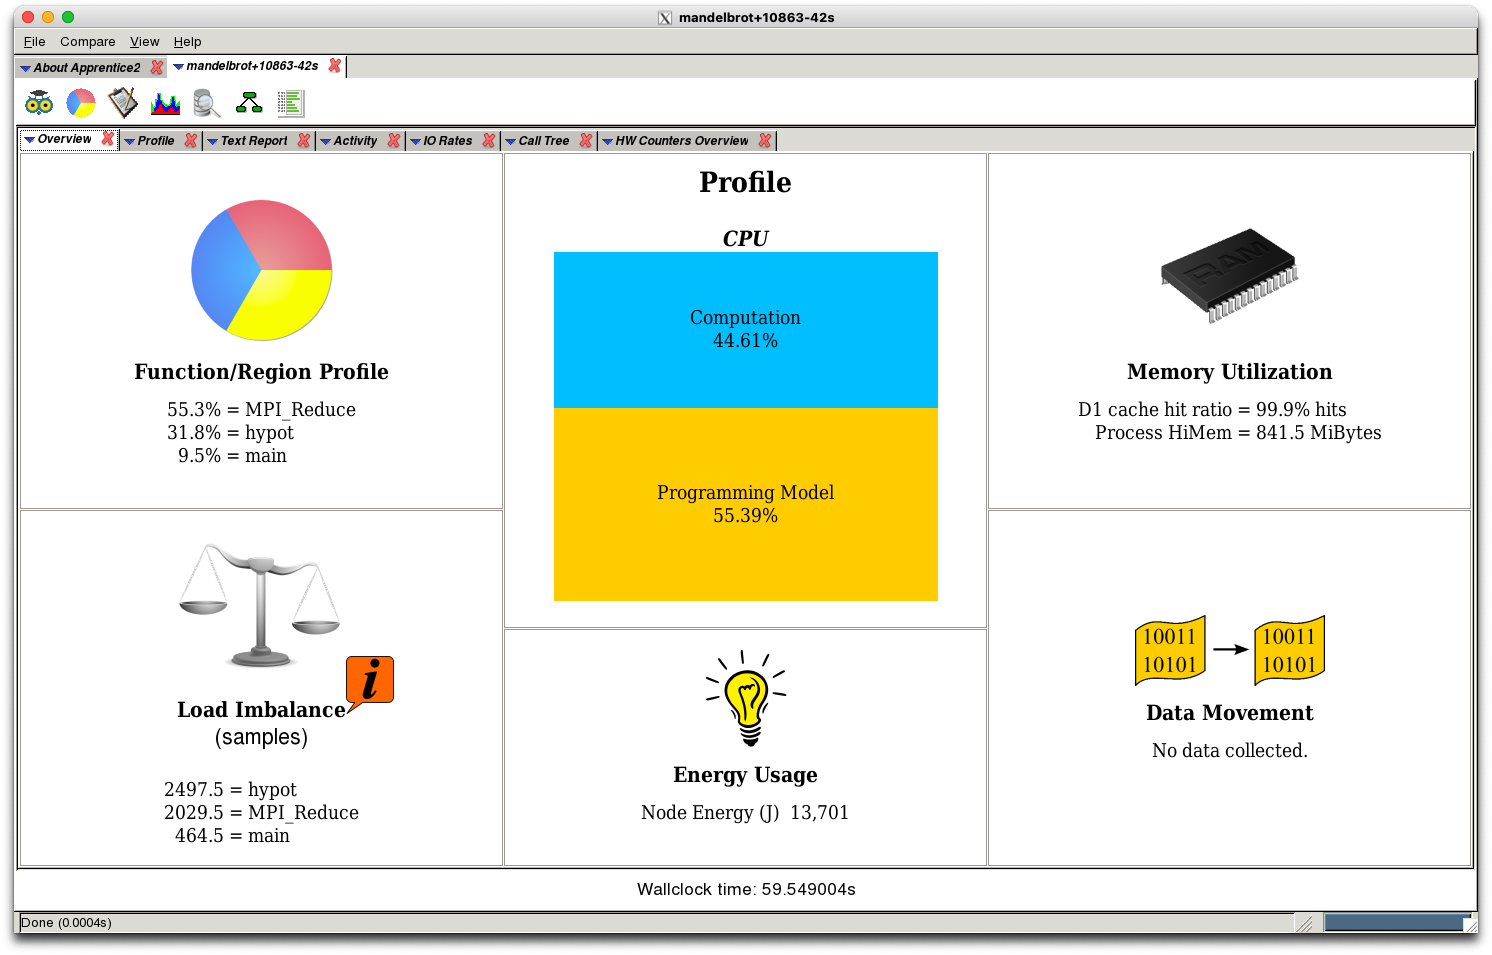
\includegraphics[scale=0.3]{figures/app2_summary}
\caption{Apprentice 2 overview window from \texttt{pertools-lite} profiling of test 1. A large fraction of time is spent in the Programming Model which indicates a performance problem.}
\label{fig:app2_summary}
\end{center}
\end{figure}
There is a clear indication of a performance problem shown by a large fraction of time is spent in the Programming Model which in this case is MPI. Looking at the sample profile pie chart (figure~\ref{fig:app2_pie} we see that around 55\% of the samples were in \texttt{MPI\_Reduce}.
\begin{figure}[htbp]
\begin{center}
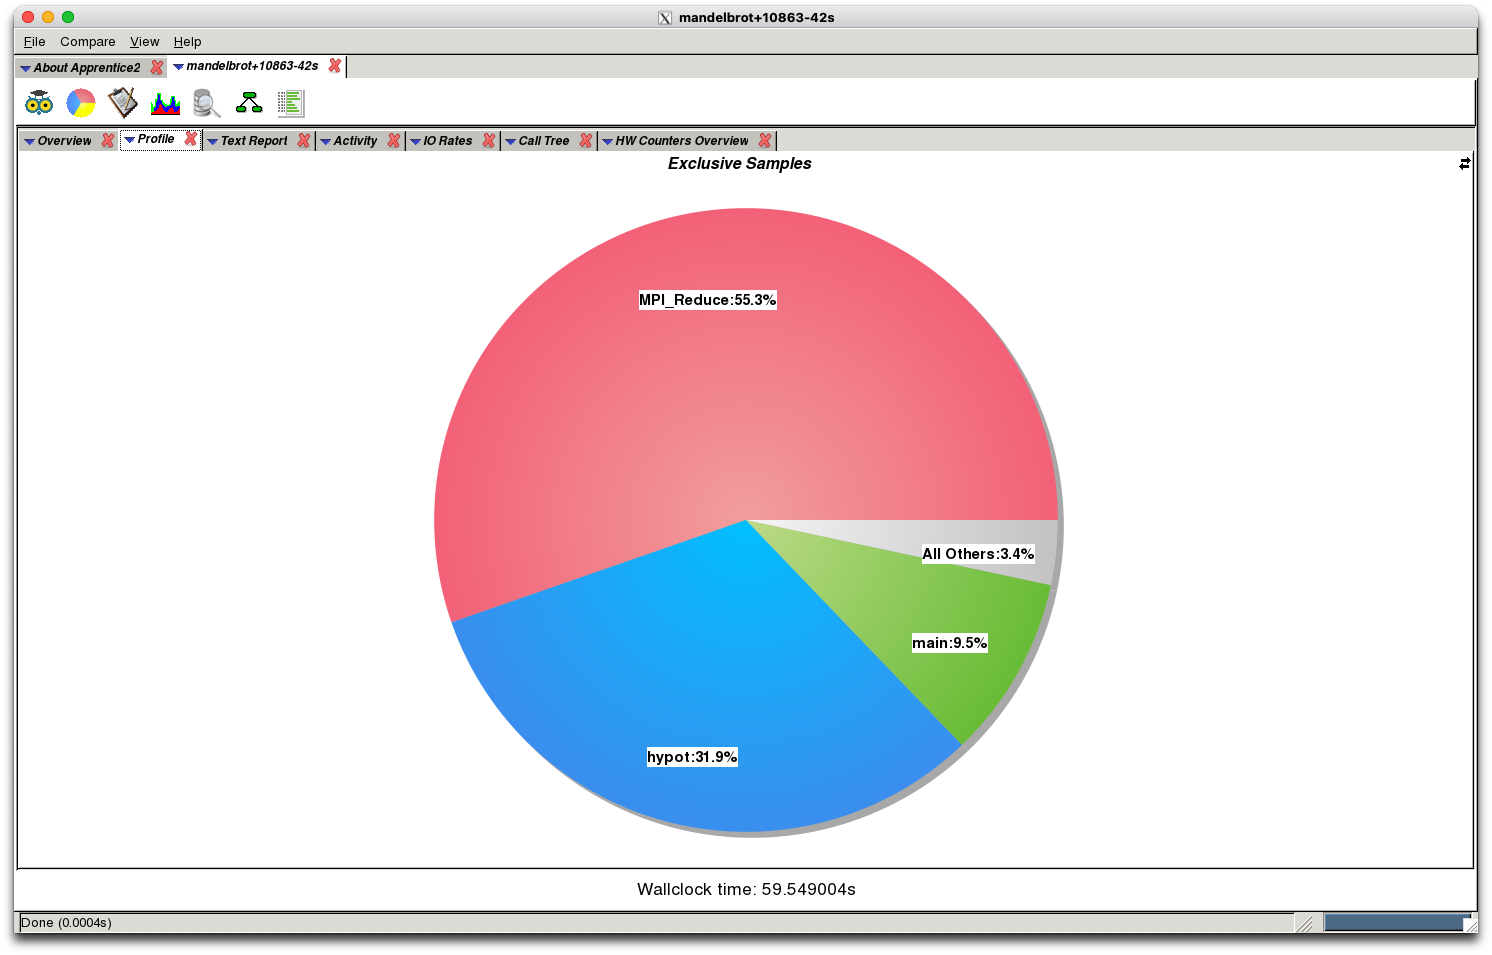
\includegraphics[scale=0.3]{figures/app2_pie}
\caption{Apprentice 2 sample profile window from \texttt{pertools-lite} profiling of test 1. In this window we can see that the time spent in the profiling model is due to an \texttt{MPI\_Reduce}.}
\label{fig:app2_pie}
\end{center}
\end{figure}
The activity window (see figure~\ref{fig:app2_activity}) shows a histogram of activity for each MPI process and we see significant variation in the time spent in collectives which is indicative of the load imbalance in this program.
\begin{figure}[htbp]
\begin{center}
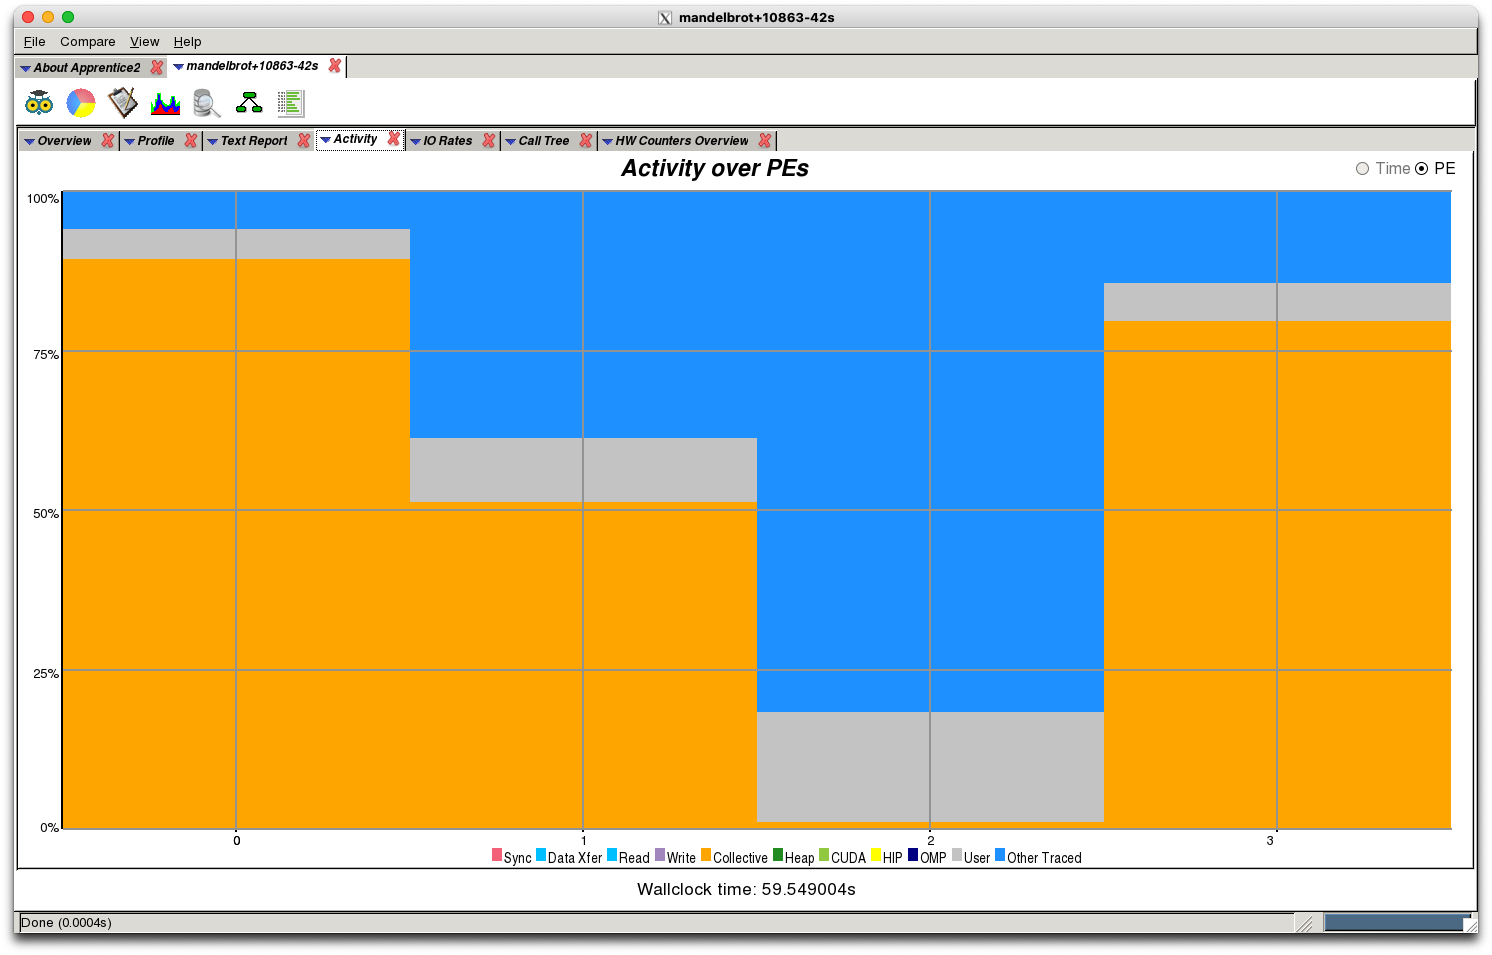
\includegraphics[scale=0.3]{figures/app2_activity}
\caption{Apprentice 2 activity window from \texttt{pertools-lite} profiling of test 1. In this window we see significant variation in the time spent in collectives which is indicative of a load imbalance.}
\label{fig:app2_activity}
\end{center}
\end{figure}
If a full trace is requested then the activity window can switch to a timeline view but this is not available with \texttt{perftools-lite}.

The full version of the profiler has many more capabilities than \texttt{perftools-lite} including viewing a time line and measuring load imbalance. To use the full capabilities of the profiler the executable is build using the \verb+pat_build+ command, the executable is run, and the profiling information generated is processed using the \verb+pat_report+ command. One feature of particular interest to the project is the ability to re-order MPI ranks to minimise network traffic by placing frequently communicating processes on the same node which could be of particular relevance when combining spatial and temporal decompositions. 

\pagebreak

%%%%%%%%%%%%%%%%%%%%%%%%%%%%%%%%%%%%%%%%%%%%%%%%%%%%%%%%%%%%%%%%%%%%%%%%%%%%%%%%%%%%%%%%%%%%%%%%%%%%%%%%%%%%%%%%%%%%%%%%%%%%%%%%%%%%%%

\section{Builds}
\label{section:builds}

There are three primary HPC platforms for the project: Isca, Isambard, Archer-2. Work on the ARCHER-2 build of Firedrake is supported by an Archer-2 eCSE project (ARCHER2-eCSE04-5 PI: Dr David A Ham (Imperial College) ``Scalable and robust Firedrake deployment on ARCHER2 and beyond'') and will not be considered further here to avoid duplication of effort.

For each target platform there is a build using the reference BLAS/Lapack implementation (fblaslapack) and optimised builds which use optimised maths libraries appropriate for the platform. The status of the builds is shown in table~\ref{table:build_status}
%
\begin{table}[htp]
\begin{center}
\begin{tabular}{|l|l|c|c|}
\hline
Platform       &  Build                   & Status         &  Profiler \\
\hline
Isca           &  GCC-OpenMPI-fblaslapack & \checkmark     &     -     \\
Isca           &  GCC-OpenMPI-OpenBLAS    & \checkmark     &     -     \\
Isca           &  Intel-IMPI-MKL          & X              &  ITAC  \\
Isambard XCI   &  GCC-CrayMPI-fblaslapack & \checkmark     & \texttt{perf-report} \\
Isambard XCI   &  GCC-CrayMPI-CrayLibsci  & \checkmark     & \texttt{perf-report} \\
\hline
\end{tabular}
\end{center}
\caption{Status of Firedrake builds and profiling for the Isca and Isambard}
\label{table:build_status}
\end{table}%

\begin{itemize}
\item Flag to PETSc can be used to switch to reference version of BLAS/Lapack
\item To see how PETSc was configured see the end of the file \texttt{firedrake/src/petsc/configure.log}

\item Vendor supplied maths libraries often have support for multi-threading which needs to be switched off when using Firedrake. Newer Firedrake versions warn about this.

\item Building Firedrake on Isca with the Intel compilers is not working because pybind11 requires Intel C++ compiler v18 or newer. 

\item The Isca build scripts are named \verb+install_firedrake_isca_COMPILER_MPI_MATHLIB.sh+
\end{itemize}

%%%%%%%%%%%%%%%%%%%%%%%%%%%%%%%%%%%%%%%%%%%%%%%%%%%%%%%%%%%%%%%%%%%%%%%%%%%%%%%%%%%%%%%%%%%%%%%%%%%%%%%%%%%%%%%%%%%%%%%%%%%%%%%%%%%%%%

\section{Profiling Firedrake}
\label{section:profiling_firedrake}

ITAC was previously working on Isca with the Intel \textbf{Say how to modify the mpirun command. Can build problems be fixed with newer compiler versions?}

ARM Forge can be used to profile python applications. Make sure to add the \verb+-j 1+ flag when using ARM profilers on Isambard otherwise there can be a hang on exit\footnote{\url{https://developer.arm.com/documentation/101136/2102/Appendix/Known-issues/Arm-MAP}} (this appears to be specific to the ARM64 architecture).

\textbf{Test with a Firedrake example e.g. high resolution DG advection. This will show point-to-point communication pattern from domain decomposition.}

It's not clear how to use Cray PAT with python/Firedrake. Loading the perftools-lite module and using the python from the cray-python module does not produce any profiling output.

%%%%%%%%%%%%%%%%%%%%%%%%%%%%%%%%%%%%%%%%%%%%%%%%%%%%%%%%%%%%%%%%%%%%%%%%%%%%%%%%%%%%%%%%%%%%%%%%%%%%%%%%%%%%%%%%%%%%%%%%%%%%%%%%%%%%%%

\section{Conclusions and recommendations}
\label{section:conclusions}

Carry out initial performance studies using Firedrake for rapid prototyping. Use ARM Forge to profile Firedrake on Isambard which enables profiling up to the 20\,992 cores. Once the scalability of the algorithm has been established on Isambard implement the algorithm in FRric and run on Archer-2 with profiling using Cray PAT. This will enable performance studies beyond 20\,000 cores.

In all cases some interpretation is needed to understand the cause of the performance problem. 

\noindent
\textbf{To do:}

\begin{enumerate}
\item Builds on Isca
\item Firedrake examples: Performance Reports/MAP, old ITAC results?
\item Write conclusions and recommendations section and describe the next steps with reference to the proposal document
\end{enumerate}

\pagebreak

%%%%%%%%%%%%%%%%%%%%%%%%%%%%%%%%%%%%%%%%%%%%%%%%%%%%%%%%%%%%%%%%%%%%%%%%%%%%%%%%%%%%%%%%%%%%%%%%%%%%%%%%%%%%%%%%%%%%%%%%%%%%%%%%%%%%%%

\section*{Appendix A}
\label{appendixA}
\begin{verbatim}
#################################################################
#                                                               #
#            CrayPat-lite Performance Statistics                #
#                                                               #
#################################################################

CrayPat/X:  Version 21.05.0 Revision 89579db89  04/08/21 23:35:55
Experiment:                  lite  lite-samples
Number of PEs (MPI ranks):      4
Numbers of PEs per Node:        4
Numbers of Threads per PE:      1
Number of Cores per Socket:    32
Execution start time:  Thu Aug  5 19:51:20 2021
System name and speed:  nid00042  2.500 GHz (nominal)
ARM   ThunderX2 (new)      CPU


Avg Process Time:          59.55 secs              
High Memory:             3,365.8 MiBytes     841.5 MiBytes per PE
Percent cycles stalled:     33.3 %          
Instr per Cycle:            1.33
I/O Write Rate:         1.164873 MiBytes/sec       

Notes for table 1:

  This table shows functions that have significant exclusive sample
    hits, averaged across ranks.
  For further explanation, see the "General table notes" below,
    or use:  pat_report -v -O samp_profile ...

Table 1:  Profile by Function

  Samp% |    Samp |    Imb. |  Imb. | Group
        |         |    Samp | Samp% |  Function=[MAX10]
        |         |         |       |   PE=HIDE
       
 100.0% | 5,940.0 |      -- |    -- | Total
|------------------------------------------------------
|  55.4% | 3,290.2 |      -- |    -- | MPI
||-----------------------------------------------------
||  55.3% | 3,284.8 | 2,029.2 | 50.9% | MPI_Reduce
||=====================================================
|  31.8% | 1,891.0 | 2,497.0 | 75.9% | MATH
||-----------------------------------------------------
||  31.8% | 1,891.0 | 2,497.0 | 75.9% | hypot
||=====================================================
|   9.5% |   562.8 |   464.2 | 60.3% | USER
||-----------------------------------------------------
||   9.5% |   562.8 |   464.2 | 60.3% | main
||=====================================================
|   3.3% |   196.0 |      -- |    -- | ETC
||-----------------------------------------------------
||   1.8% |   107.5 |   143.5 | 76.2% | __mulsc3
||   1.0% |    60.2 |    76.8 | 74.7% | __hypot_finite
|======================================================

Notes for table 2:

  This table shows functions, and line numbers within functions, that
    have significant exclusive sample hits, averaged across ranks.
  For further explanation, see the "General table notes" below,
    or use:  pat_report -v -O samp_profile+src ...

Table 2:  Profile by Group, Function, and Line

  Samp% |    Samp |    Imb. |  Imb. | Group
        |         |    Samp | Samp% |  Function=[MAX10]
        |         |         |       |   Source
        |         |         |       |    Line
        |         |         |       |     PE=HIDE
       
 100.0% | 5,940.0 |      -- |    -- | Total
|-----------------------------------------------------------------------------
|  55.4% | 3,290.2 |      -- |    -- | MPI
||----------------------------------------------------------------------------
||  55.3% | 3,284.8 | 2,029.2 | 50.9% | MPI_Reduce
||============================================================================
|  31.8% | 1,891.0 | 2,497.0 | 75.9% | MATH
||----------------------------------------------------------------------------
||  31.8% | 1,891.0 | 2,497.0 | 75.9% | hypot
||============================================================================
|   9.5% |   562.8 |      -- |    -- | USER
||----------------------------------------------------------------------------
||   9.5% |   562.8 |      -- |    -- | main
3|        |         |         |       |  PAT_test/runs/test1/mandelbrot_mpi.c
||||--------------------------------------------------------------------------
4|||   2.4% |   144.0 |   155.0 | 69.1% | line.85
4|||   2.0% |   120.8 |   166.2 | 77.2% | line.87
||||==========================================================================
||============================================================================
|   3.3% |   196.0 |      -- |    -- | ETC
||----------------------------------------------------------------------------
||   1.8% |   107.5 |      -- |    -- | __mulsc3
3|        |         |         |       |  ../cray-gcc-9.3.0-202003310324.b29d417121fbe/libgcc/libgcc2.c
||   1.0% |    60.2 |    76.8 | 74.7% | __hypot_finite
|=============================================================================

Observation:  MPI utilization

    No suggestions were made because all ranks are on one node.


Notes for table 3:

  This table shows energy and power usage for the nodes with the
    maximum, mean, and minimum usage, as well as the sum of usage over
    all nodes.
    Energy and power for accelerators is also shown, if applicable.
  For further explanation, see the "General table notes" below,
    or use:  pat_report -v -O program_energy ...

Table 3:  Program energy and power usage (from Cray PM)

   Node |     Node |   Process | PE=HIDE
 Energy |    Power |      Time | 
    (J) |      (W) |           | 
----------------------------------------
 13,701 |  230.085 | 59.547615 | Total
========================================

Notes for table 4:

  This table show the average time and number of bytes written to each
    output file, taking the average over the number of ranks that
    wrote to the file.  It also shows the number of write operations,
    and average rates.
  For further explanation, see the "General table notes" below,
    or use:  pat_report -v -O write_stats ...

Table 4:  File Output Stats by Filename

      Avg |      Avg |  Write Rate | Number |    Avg | Bytes/ | File Name=!x/^/(proc|sys)/
    Write |    Write | MiBytes/sec |     of | Writes |   Call |  PE=HIDE
 Time per |  MiBytes |             | Writer |    per |        | 
   Writer |      per |             |  Ranks | Writer |        | 
     Rank |   Writer |             |        |   Rank |        | 
          |     Rank |             |        |        |        | 
|-----------------------------------------------------------------------------
| 0.000051 | 0.000059 |    1.164873 |      1 |    2.0 |  31.00 | stdout
|=============================================================================
Program invocation:  ./mandelbrot

For a complete report with expanded tables and notes, run:
  pat_report /lustre/home/user/PAT_test/runs/test1/mandelbrot+10863-42s

For help identifying callers of particular functions:
  pat_report -O callers+src /lustre/home/user/PAT_test/runs/test1/mandelbrot+10863-42s
To see the entire call tree:
  pat_report -O calltree+src /lustre/home/user/PAT_test/runs/test1/mandelbrot+10863-42s

For interactive, graphical performance analysis, run:
  app2 /lustre/home/user/PAT_test/runs/test1/mandelbrot+10863-42s

================  End of CrayPat-lite output  ==========================
\end{verbatim}



\end{document}
